\documentclass[12pt,a4paper]{article}
\usepackage{amsmath}
\usepackage{amsfonts}
\usepackage{amssymb}
\usepackage{makeidx}
\usepackage{graphicx}
\usepackage{wrapfig}
\usepackage{enumerate}
\usepackage{pdfpages}
\usepackage{tocloft}
\usepackage{setspace}
\usepackage{mathtools}
\usepackage{hyperref}
\definecolor{linkcolour}{rgb}{0,0.2,0.6} % Link color
\hypersetup{colorlinks,breaklinks,urlcolor=linkcolour,linkcolor=linkcolour}
\usepackage[left=2cm,right=2cm,top=2cm,bottom=2cm]{geometry}

\usepackage{xcolor}
\usepackage{fontspec}
\setmainfont{Cambria}

\usepackage{subcaption}
\usepackage{caption}
\captionsetup[figure]{font=small, labelfont={bf}}
\captionsetup[table]{font=small, labelfont={bf}}

\usepackage{float}
\usepackage{multirow}
\usepackage{longtable}
\usepackage[nottoc]{tocbibind}

\usepackage{soul}

\newcommand{\spa}{\vspace{1.25em}}
\newcommand{\noi}{\noindent}
\def\dul#1{\underline{\underline{#1}}}
\def\cpt#1#2{{\begin{center}\small\textbf{\textcolor{blue}{Figure #1:}} #2\end{center}}}
\def\tt#1{\texttt{#1}}
% for dots in the content
\usepackage{tocloft}
\renewcommand{\cftsecleader}{\cftdotfill{\cftdotsep}}

% For getting paragraphs
\usepackage{titlesec}
\setcounter{secnumdepth}{4}
\setcounter{tocdepth}{4}
\titleformat{\paragraph}
{\normalfont\normalsize\bfseries}{\theparagraph}{1em}{}
\titlespacing*{\paragraph}
{0pt}{3.25ex plus 1ex minus .2ex}{1.5ex plus .2ex}


\begin{document}
    \begin{titlepage} 
        \begin{center}
        \large{ASSIGNMENT 1}\\
        \vspace{2em}
        \large {CS5691 Pattern Recognition and Machine Learning}
        \vspace{3em}
        
        \rule{0.9\linewidth}{0.5mm} \\[0.4cm]
        {\Large{\bfseries{CS5691 Assignment 1}}} \\
        \rule{0.9\linewidth}{0.5mm} \\[3 em]    
        
        Team Members: \\
        \vspace{0.5em}
        \def\arraystretch{1.25}
\begin{tabular}{c l}
	\hline
	BE17B007 & N Sowmya Manojna \\
	PH17B010 & Thakkar Riya Anandbhai \\
	PH17B011 & Chaithanya Krishna Moorthy \\
	\hline
\end{tabular}

        \vspace{1em}

        Indian Institute of Technology, Madras\\    
        
        \vspace{5em}    
        
            
\includegraphics[scale = 0.09]{images/iitmlogo.png}
        \end{center}
    \end{titlepage}
{\hypersetup{linkcolor=black}
\tableofcontents}
\break

\section{Task 1}
\subsection{Mathematical Formulation}
The data for univariate polynomial regression is obtained by raising it to the required degree. In case of univariate polynomial regression of degree $d$, the dependent variable, of size $(d,1)$ is assumed to have the form
\begin{equation}
    \vec{y}_{n\times1} = \mathit{\phi}_{n\times d}W_{d\times1}
\end{equation}
\noi
The weights corresponding to a given degree is then calculated by using the closed form solution for univariate polynomial regression:
\begin{equation}
    W = (\mathit{\phi}^T\mathit{\phi} + \lambda \mathit{I})^{-1}\mathit{\phi}^T\vec{y}
\end{equation}
Where, $\lambda\mathit{I}$ is the regularization term.

\subsection{Training and Validation Accuracies}
In order to pick the parameters that best fit the dataset, a grid search was performed on the dataset. Prior to this, the dataset was split into training set, validation set and the testing set, in the ratio 70:10 (from the training data) :30. The results obtained is as follows:\\

\begin{minipage}{0.4\textwidth}
\def\arraystretch{1.25}
\begin{center}
{\small
\begin{longtable}{l l l l l}
\hline
\hline
\textbf{$d$} & \textbf{$\lambda$} & \textbf{Train Error} & \textbf{Validation Error} \\
\hline
\hline
6 & 0.0 & 0.044889 & 0.159636 \\
3 & 0.0 & 0.672882 & 1.001484 \\
9 & 0.5 & 0.750020 & 1.469413 \\
2 & 0.0 & 1.014199 & 1.883134 \\
9 & 1.0 & 1.040132 & 1.929033 \\
9 & 2.0 & 1.354363 & 2.165779 \\
9 & 10.0 & 2.281929 & 1.857270 \\
9 & 50.0 & 3.342110 & 1.447933 \\
9 & 100.0 & 3.782560 & 1.380623 \\
9 & 0.0 & 5.063475 & 92.085167 \\
\hline
\caption{Results obtained for Task 1, with sample size of 10}
\end{longtable}
}
\end{center}
\end{minipage}\hfill%
\begin{minipage}{0.4\textwidth}
\def\arraystretch{1.25}
\begin{longtable}{l l l l l}
\hline
\hline
\textbf{Degree} & \textbf{$\lambda$} & \textbf{Train Error} & \textbf{Validation Error} \\
\hline
\hline
6 & 0.0 & 0.094536 & 0.094379 \\
9 & 0.0 & 0.093581 & 0.100752 \\
9 & 0.5 & 0.134226 & 0.152565 \\
9 & 1.0 & 0.186479 & 0.209008 \\
9 & 2.0 & 0.289107 & 0.311716 \\
9 & 10.0 & 0.766298 & 0.776521 \\
3 & 0.0 & 0.934079 & 0.862605 \\
2 & 0.0 & 1.591842 & 1.421021 \\
9 & 50.0 & 1.620063 & 1.707757 \\
9 & 100.0 & 2.138200 & 2.310223 \\
\hline
\caption{Results obtained for Task 1, with sample size of 200}
\end{longtable}
\end{minipage}%

\vspace{1em}
\noi
Regularization was only applied in case of degree 9.\\

\noi
\textcolor{blue}{From the table above, we see that the best fit for the data is obtained for degree: $6$ and $\lambda:0$.}

\subsection{Model Fits}
\subsubsection{Sample Size: 10}
The polynomial models and the corresponding fits obtained for sample size of 10 are as follows:
\begin{figure}[H]
    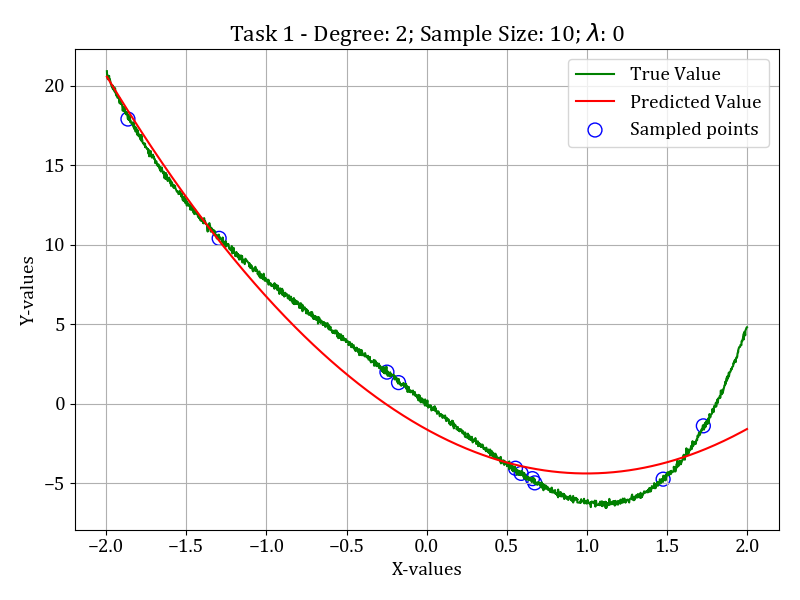
\includegraphics[scale=0.425]{images/t1_d1/d_2_size_10_l_0.png}
    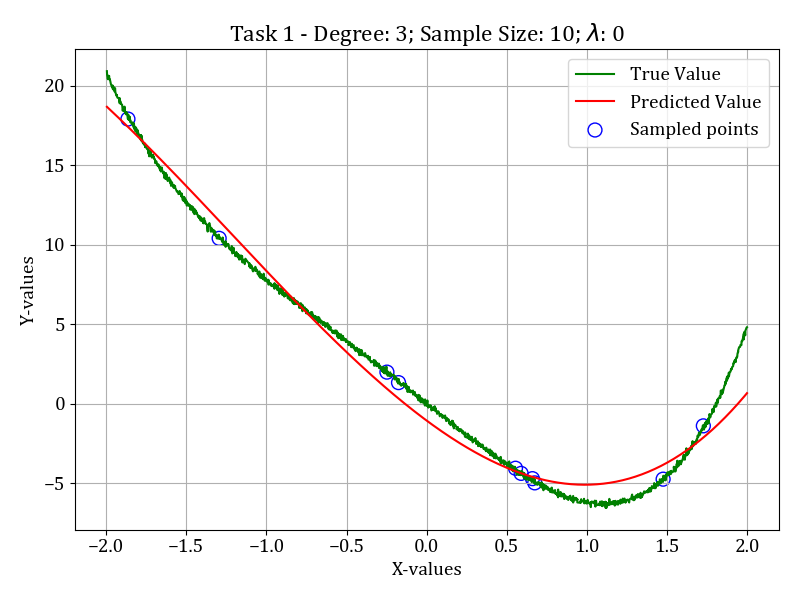
\includegraphics[scale=0.425]{images/t1_d1/d_3_size_10_l_0.png}
    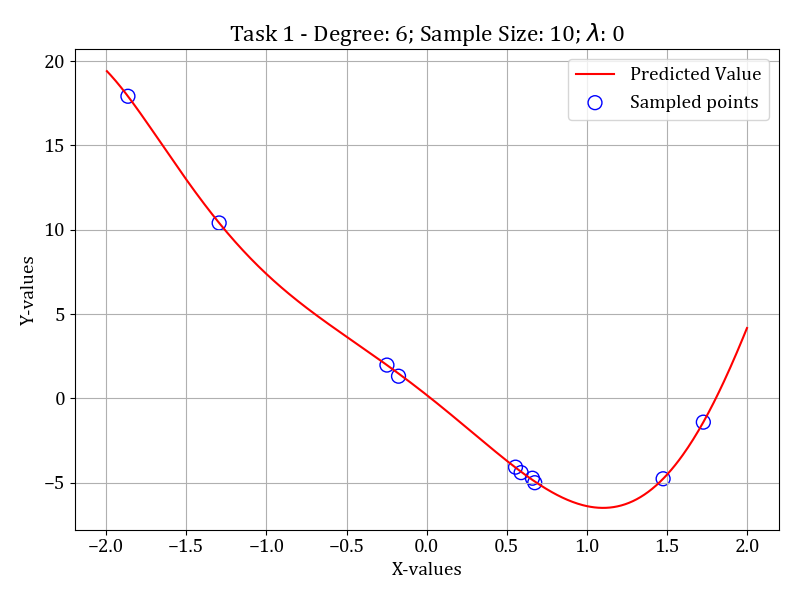
\includegraphics[scale=0.425]{images/t1_d1/d_6_size_10_l_0.png}
    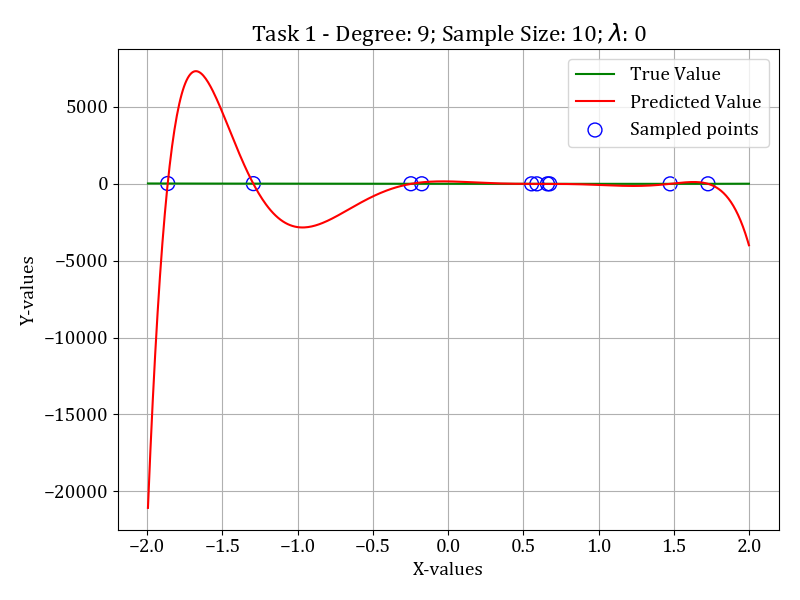
\includegraphics[scale=0.425]{images/t1_d1/d_9_size_10_l_0.png}
    \caption{Task 1 - Polynomial fits, Sample size: 10}
\end{figure}

\paragraph{Inference}
From the above plots, we can see that:
\begin{itemize}
    \itemsep0em
    \item Lower degree polynomial curves aren't able to model the dataset well (i.e.) the curve doesn't pass through all the data points.
    \item Higher degree polynomials are able to fit the dataset well. The curves pass through all the data points.
    \item However, the polynomial degree 9 curve has a large variance along the y-axis than the remaining polynomial degrees.
\end{itemize}

\subsubsection{Sample Size: 200}
The polynomial models and the corresponding fits obtained for sample size of 200 are as follows:
\begin{figure}[H]
    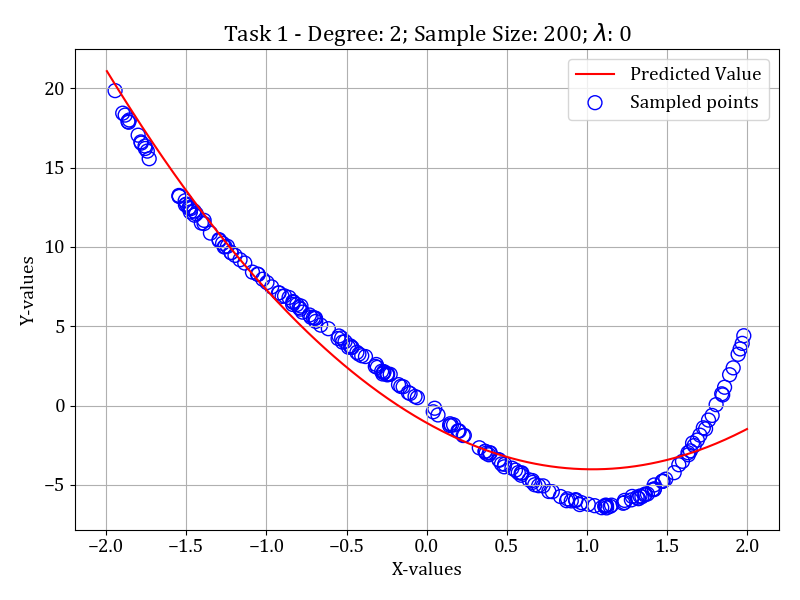
\includegraphics[scale=0.425]{images/t1_d1/d_2_size_200_l_0.png}
    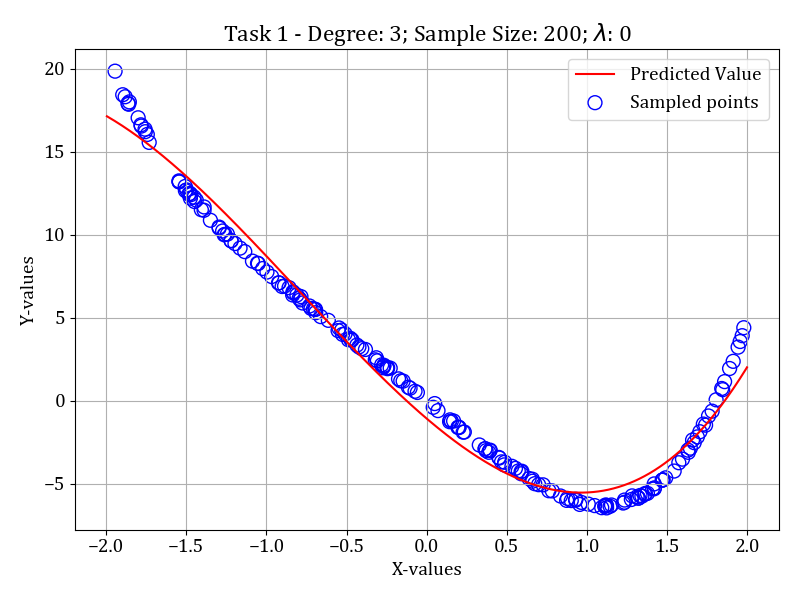
\includegraphics[scale=0.425]{images/t1_d1/d_3_size_200_l_0.png}
    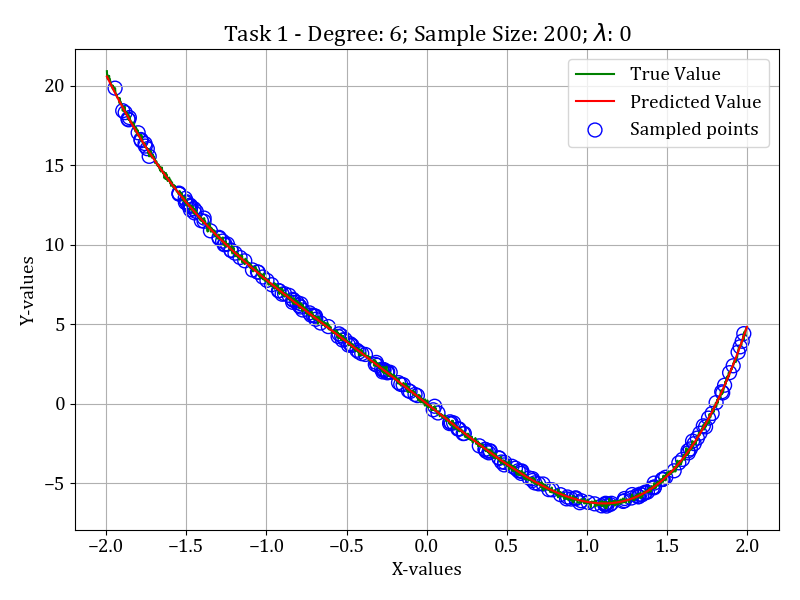
\includegraphics[scale=0.425]{images/t1_d1/d_6_size_200_l_0.png}
    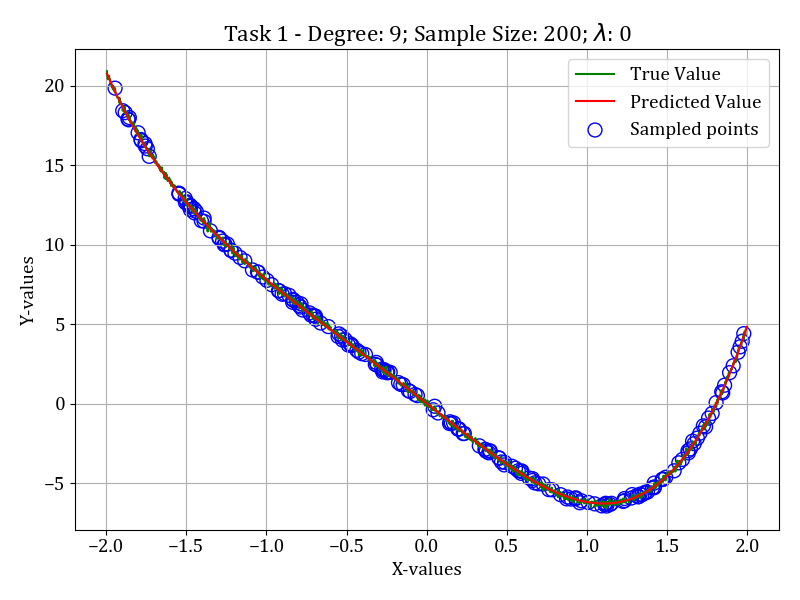
\includegraphics[scale=0.425]{images/t1_d1/d_9_size_200_l_0.png}
    \caption{Task 1 - Polynomial fits, Sample size: 200}
\end{figure}

\paragraph{Inference}
From the above plots, we can see that:
\begin{itemize}
    \itemsep0em
    \item Lower degree polynomial curves aren't able to model the dataset well (i.e.) the curve doesn't pass through all the data points.
    \item Higher degree polynomials are able to fit the dataset well. The curves pass through all the data points.
    \item We can see a clear difference between the degree 9 fit when the dataset size was 10 to that when the dataset size is 200. The increase in dataset size helped decrease the variance and overfitting.
\end{itemize}

\subsubsection{Effects of Regularization}
The polynomial models and the corresponding fits obtained for degree 9, sample size of 10, across different $\lambda$ values are as follows:
\begin{figure}[H]
    \hspace{-2em}
    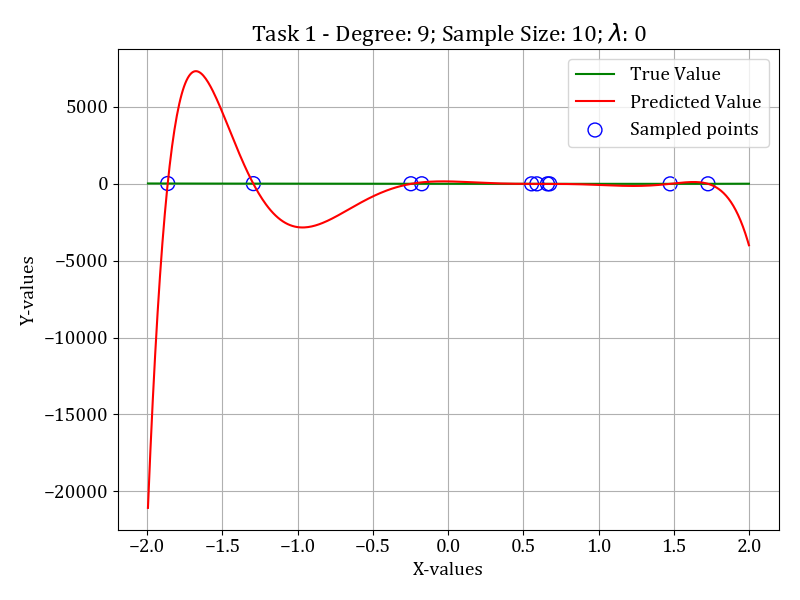
\includegraphics[scale=0.45]{images/t1_d1/d_9_size_10_l_0.png}
    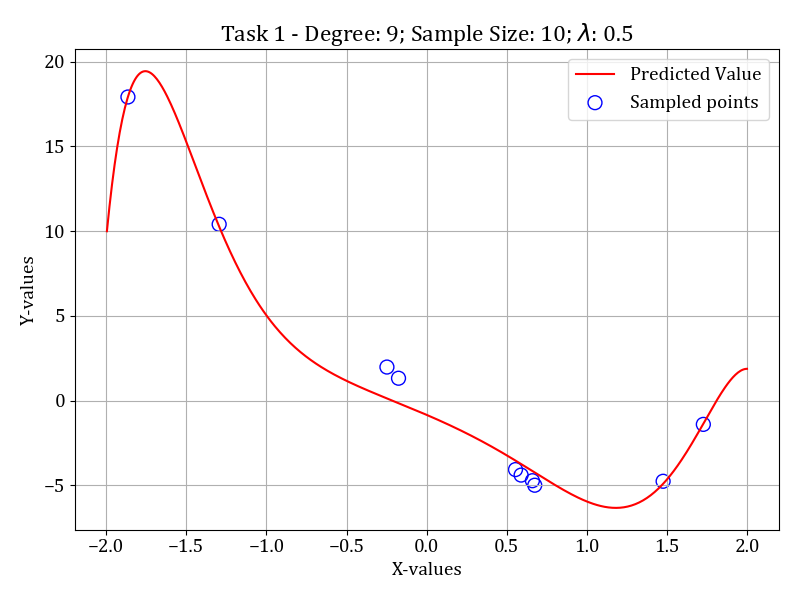
\includegraphics[scale=0.45]{images/t1_d1/d_9_size_10_l_0.5.png}
\end{figure}
\begin{figure}[H]
    \vspace{-2em}
    \hspace{-2em}
    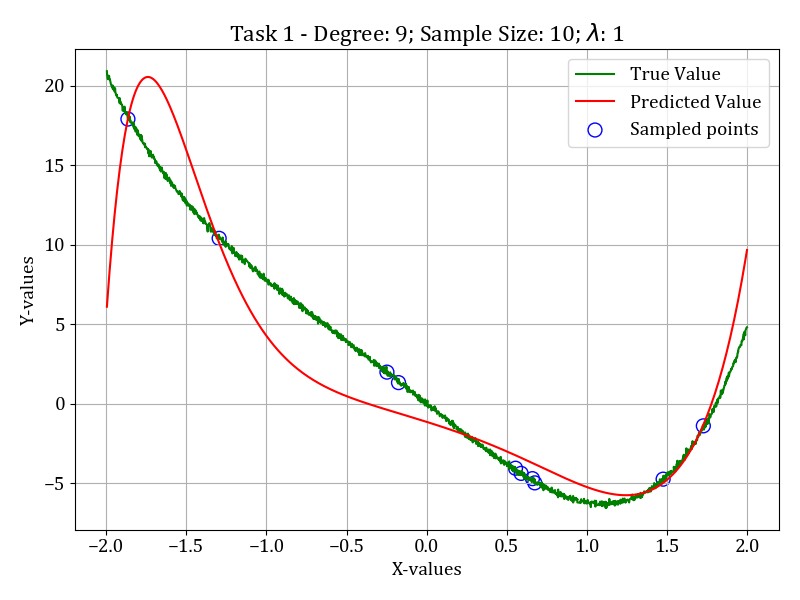
\includegraphics[scale=0.45]{images/t1_d1/d_9_size_10_l_1.png}
    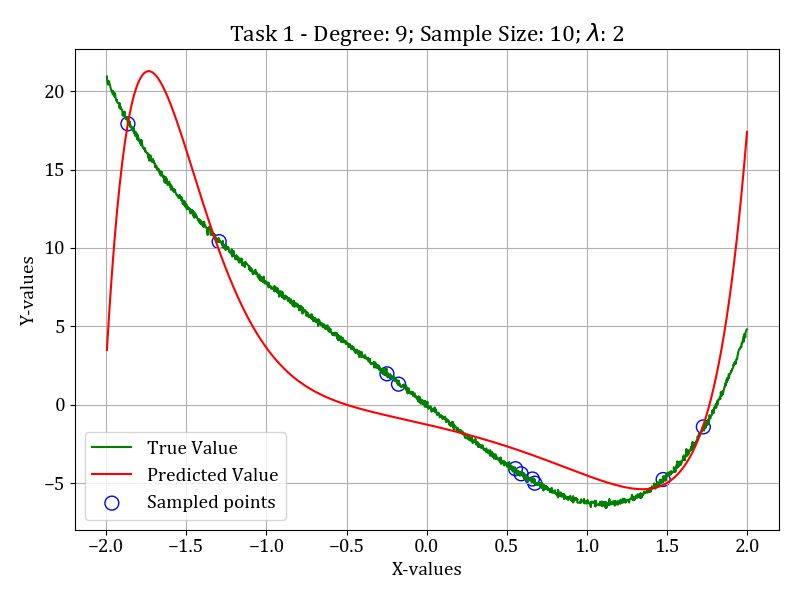
\includegraphics[scale=0.45]{images/t1_d1/d_9_size_10_l_2.png}
\end{figure}
\begin{figure}[H]
    \vspace{-2em}
    \hspace{-2em}
    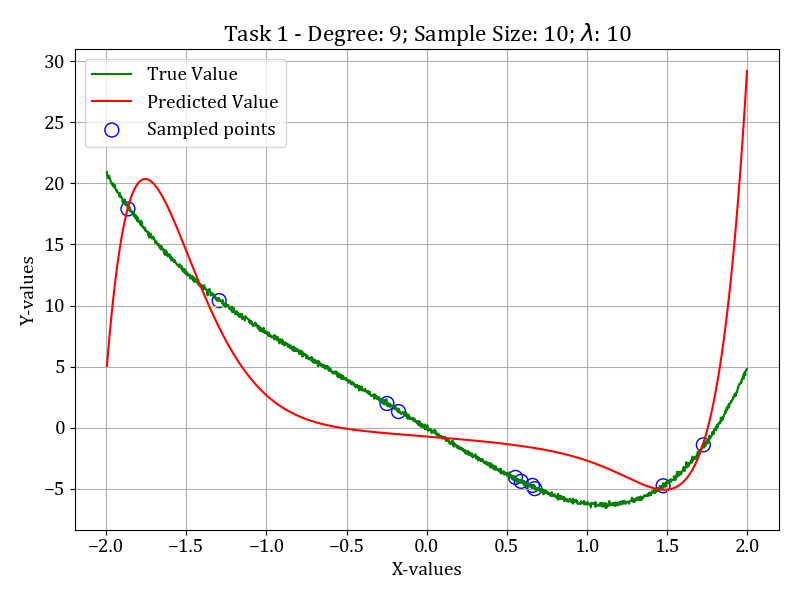
\includegraphics[scale=0.45]{images/t1_d1/d_9_size_10_l_10.png}
    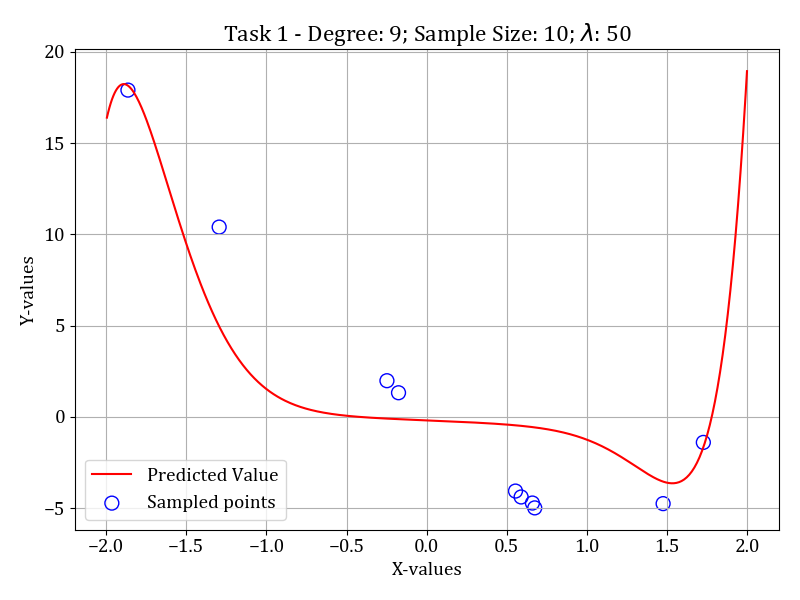
\includegraphics[scale=0.45]{images/t1_d1/d_9_size_10_l_50.png}
\end{figure}
\begin{figure}[H]
    \vspace{-2em}
    \centering
    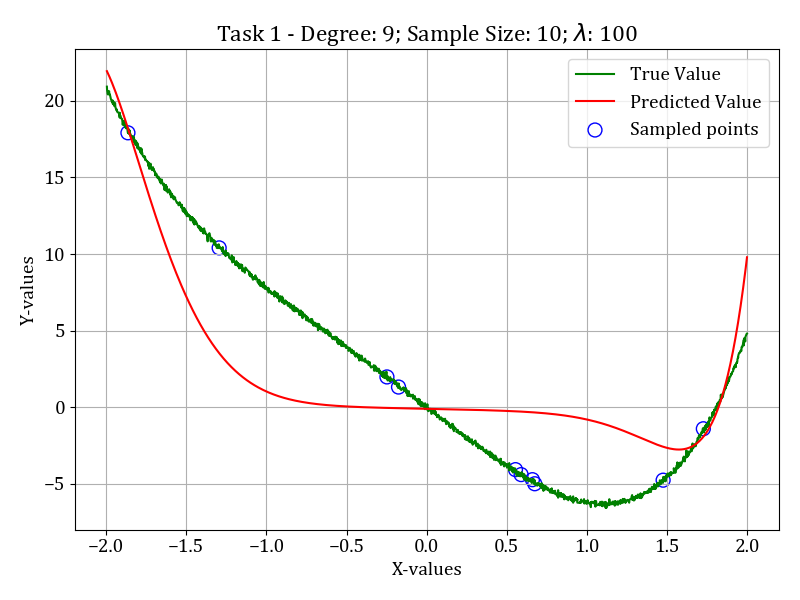
\includegraphics[scale=0.45]{images/t1_d1/d_9_size_10_l_100.png}
    \caption{Task 1 - 9\textsuperscript{th} Degree Polynomial fit, Sample size: 10}
\end{figure}

\paragraph{Inference}
From the above plots, we can see that:
\begin{itemize}
    \itemsep0em
    \item Regularization was only applied to the degree 9 polynomial, with 10 data points as it had the same number of data points and parameters. 
    \item We can see that, the curve starts becoming more flatter with increasing value of the  regularization parameter $\lambda$.
    \item This could be because, the weights corresponding to higher degrees became smaller.
\end{itemize}

\subsection{Best Model}
The best fit, $d:6$ and $\lambda:0$ is visualized as follows:
\begin{figure}[H]
    \hspace{-2em}
    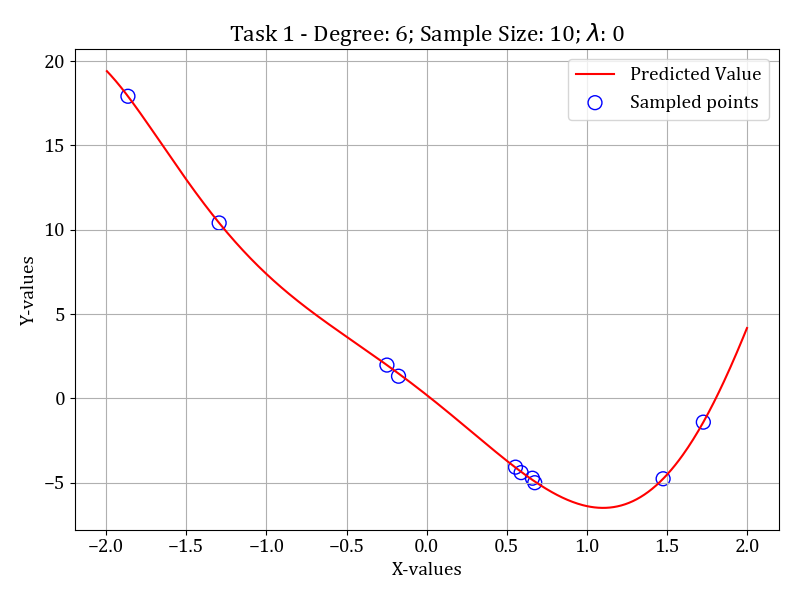
\includegraphics[scale=0.45]{images/t1_d1/d_6_size_10_l_0.png}
    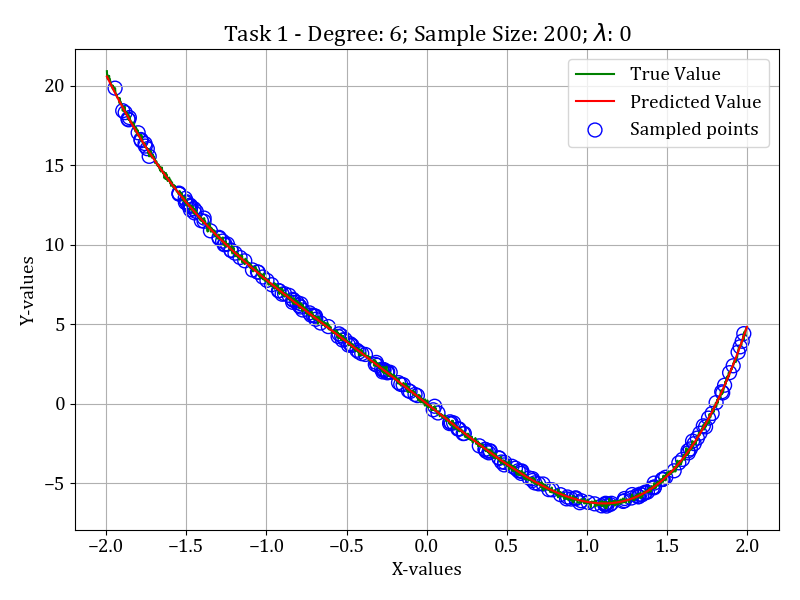
\includegraphics[scale=0.45]{images/t1_d1/d_6_size_200_l_0.png}
    \caption{Task 1 - Best fit, Sample size: 10 (to the left) and Sample size: 200 (to the right)}
\end{figure}

\noi
\textcolor{blue}{
The training and testing error obtained from the best model is as follows:
\begin{itemize}
    \itemsep0em
    \item Training Error: $0.09974659089780814$
    \item Testing Error: $0.09793071099285168$
\end{itemize}
}

\section{Task 2}
\subsection{Mathematical Formulation}
The dataset allotted to our group for task 2 is \tt{function1\_2d.csv}, which has a 2 dimensional feature vector and 1 dimensional target output to be predicted. We assume that the target variable is of the form:

\begin{equation}
\label{eq:1}
    y=\sum_{i=0}\omega _{i}\phi_{i}(x_1,x_2)  +\epsilon 
\end{equation}

\noi
Where $\omega_{i}$ are the parameters to be found through regression, $\phi_{i}(x1,x2)$ is a polynomial in $x_1$ and $x_2$ and $\epsilon$ is the normally distributed error. 
\\ 

\noi
A breakdown of the steps undertaken is:
\begin{itemize}
    \itemsep0em
    \item The function \tt{create\_phi} generates the design matrix $\phi(x1,x2)$ for the required degree of complexity.
    The number of attributes in the generated design matrix is given by:
    \begin{equation}
        D=\frac{(M+d)!}{M!\,d!}
    \end{equation}
    where d is the dimension of the original feature vector (=2 for Task 2) and M is the degree of complexity of the model.
    \item To avoid overfitting, as a general rule $\tt{N}>10*D$
    \item The design matrix is passed to the function \tt{regularized\_pseudo\_inv} , which generates the Moore-Penrose inverse of the given design matrix(X) and specified value of regularization parameter lambda($\lambda$).
    
    \begin{equation}
         (\lambda I+X^{T}X)^{-1}X^{T}
    \end{equation}
    
    \item The function \tt{opt\_regularized\_param} is then used to obtain optimum values of $\vec{\omega}$
    \begin{equation}
        \vec{\omega} = [(\lambda I+X^{T}X)^{-1}X^{T}].y
    \end{equation}
    Where $y$ is the output as defined in the \autoref{eq:1}.
    
    \item The optimum parameter vector thus obtained can be used to predict the variable y for new inputs. 
    \begin{equation}
        y_{prediction}=X\vec{\omega}
    \end{equation}
\end{itemize}

The results obtained for various degrees of complexities are discussed below. 

\subsection{Degree of complexity: 2}
With degree of complexity set to 2, the number of parameters in our model are:
\begin{equation}
\begin{split}
 D &= \frac{(d+M)!}{d!\,M!} \\
   & =\frac{(4!)}{2!\,2!} \\
   & =6
\end{split}
\end{equation}

\noi
Since the number of parameters to be estimated is very less compared to our sample sizes, we do not expect to see over fitting, and hence regularization is not used. 

\subsubsection{Surface plots of Approximated function}
Surface plots obtained for various train sizes are as follows: 
\begin{figure}[H]
    \centering
    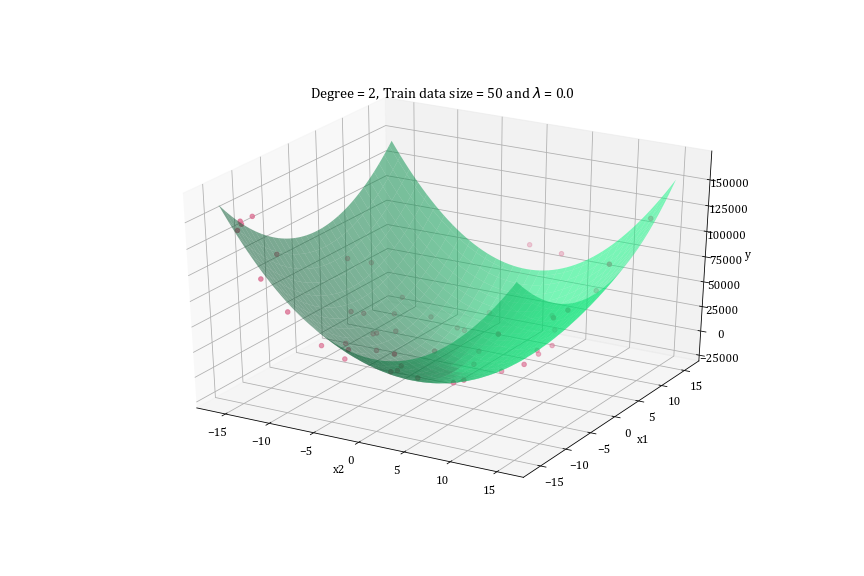
\includegraphics[scale=0.6]{images/D=2,T=50,l=0.0.png}
    \hspace{2em}
    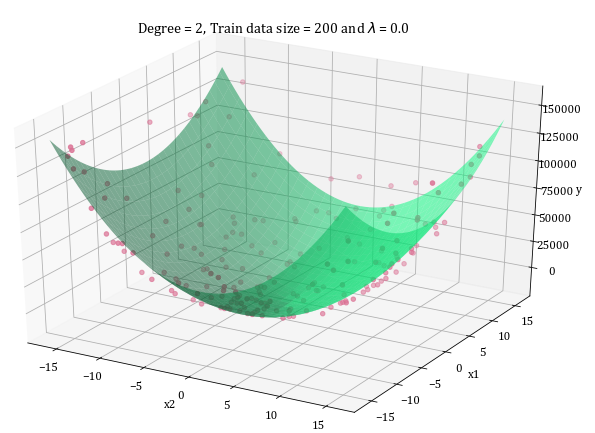
\includegraphics[scale=0.6]{images/D=2,T=200,l=0.0.png}
    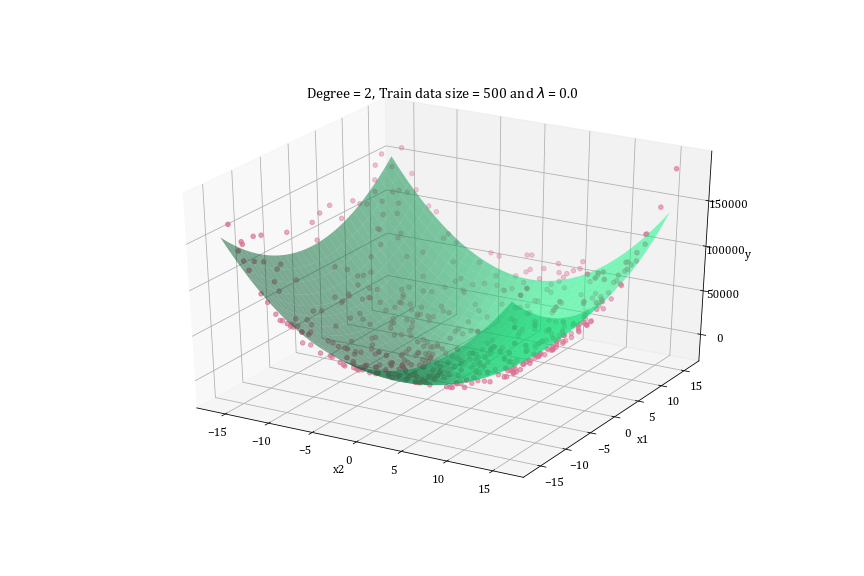
\includegraphics[scale=0.6]{images/D=2,T=500,l=0.0.png}
    \caption{Surface Plot of the approximated function for different training sizes, Degree: 2}
    \label{fig:sp_d2}
\end{figure}

\subsubsection{Erms over Train, Validation and Test data}
The $E_{rms}$ over train, validation and test data is obtained to be: 
\def\arraystretch{1.25}
\begin{table}[H]
\centering
\begin{tabular}{l l l l l}
\hline
\hline
\textbf{Train size} & \textbf{$\lambda$} & \textbf{Erms Train} & \textbf{Erms Validation} & \textbf{Erms Test}\\
\hline
\hline
50 & 0 & 9.34*$10^3$ & 1.06*$10^4$ & 1.14*$10^4$  \\
200 & 0 & 1.06*$10^4$ & 1.14*$10^4$ & 1.15*$ 10^4$  \\
500 & 0 & 1.13*$10^4$ & 1.12*$10^4$ & 1.08*$10^4$\\
\hline
\end{tabular}
\caption{Erms for different train sizes for degree of complexity 2}
\end{table}


\subsubsection{Inference}
\begin{itemize}
    \itemsep0em
    \item While the magnitude of $E_{rms}$ is nearly same over train, validation and test data, it does not reduce on increasing the sample size. 
    \item The surface plot of approximated function is simple and poorly fits both the training as well as test data.
    \item From the above two points, we conclude that we have an oversimplified model with a high bias. Increasing the complexity would be beneficial.
\end{itemize}

\subsection{Degree of complexity: 3}
The number of parameters to be estimated for this model are: 
\begin{equation}
    \begin{split}
        D&=\frac{(2+3)!}{2!\,3!} \\
         &=10
    \end{split}
\end{equation}

\noi
Since for train data size $50, 50<10*10$, we apply regularization. As reported in the $E_{rms}$ table, the errors increases on applying regularization. Regularization need not be applied for train data size 200 and 500. 

\subsubsection{Surface plots of the approximated function}
The surface plots of approximated function for various train data sizes is: 

\begin{figure}[H]
    \centering
    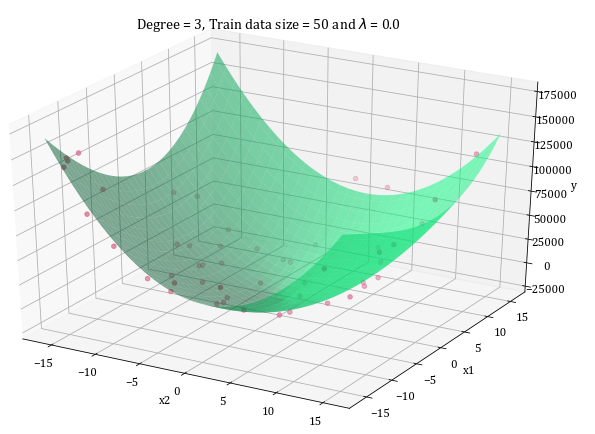
\includegraphics[scale=0.6]{images/D=3,T=50,l=0.0.png}
    \hspace{2em}
    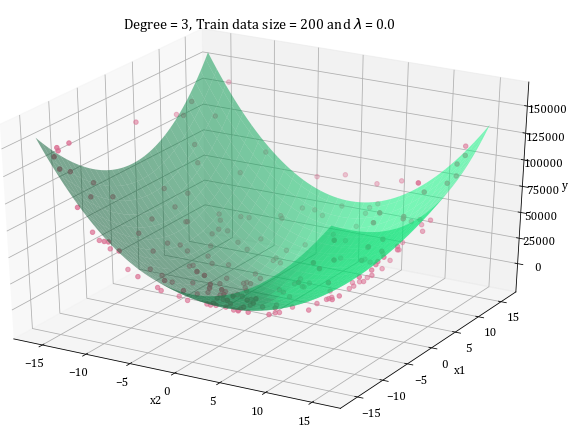
\includegraphics[scale=0.6]{images/D=3,T=200,l=0.0.png}
    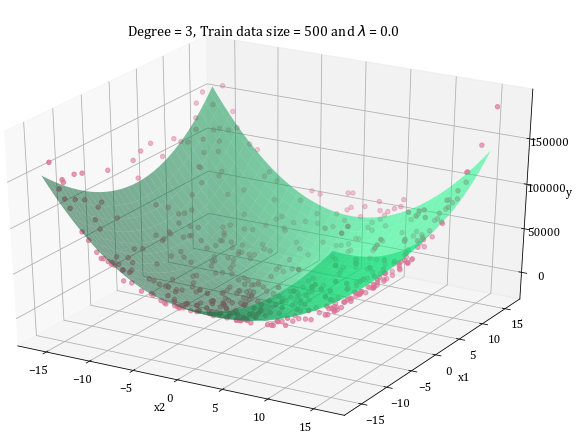
\includegraphics[scale=0.6]{images/D=3,T=500,l=0.0.png}
    \caption{Surface plot of approximated function for different train sizes, Degree: 3}
    \label{fig:sp_d3}
\end{figure}

\subsubsection{Erms over Train, Validation and Test data}
The $E_{rms}$ over Train, Validation and Test data is obtained to be:
\def\arraystretch{1.25}
\begin{table}[H]
\centering
\begin{tabular}{l l l l l}
\hline
\hline
\textbf{Train size} & \textbf{$\lambda$} & \textbf{Erms Train} & \textbf{Erms Validation} & \textbf{Erms Test}\\
\hline
\hline
50 & 0 & 8.40*$10^3$ & 1.19*$10^4$ & 1.23*$10^4$  \\
50 & 1 & 8.43*$10^3$ & 1.19*$10^4$ & 1.22*$10^4$ \\
50 & 10 & 9.24*$10^3$ & 1.07*$10^3$ & 1.31*$10^4$ \\
200 & 0 & 1.03*$10^4$ & 1.14*$10^4$ & 1.15*$ 10^4$  \\
500 & 0 & 1.11*$10^4$ & 1.11*$10^4$ & 1.11*$10^4$\\
\hline
\end{tabular}
\caption{Erms for different train sizes for degree of complexity 3}
\end{table}



\subsubsection{Inference}
\begin{itemize}
    \itemsep0em
    \item The $E_{rms}$ values are nearly same as that for degree of complexity 2.
    \item Increasing the sample size does not affect the $E_{rms}$ significantly.
    \item While $E_{rms}$ Train is lower for sample size 50, it is due to inadequate number of data samples. $E_{rms}$ Train, $E_{rms}$ Validation and $E_{rms}$ Test converge as the train data size increases to 500.
    \item From the above points we conclude that this model too is oversimplified and thus fails to perform well over Train, Validation as well as Test data. Our model thus has a high bias error similar to model of complexity 2. 
\end{itemize}

\subsection{Degree of complexity: 6}
The number of parameters to be estimated are-
\begin{equation}
    \begin{split}
        D&=\frac{(2+6)!}{2!\,6!} \\
        &=28
    \end{split}
\end{equation}

\noi
For train data size 50, $N<28*10$, hence regularization is applied to the model. However, regularization is not needed for training data sizes of 200 and 500. 

\subsubsection{Surface plots of the approximated function}
The surface plots of the approximated function for various train data sizes are:

\begin{figure}[H]
    \centering
    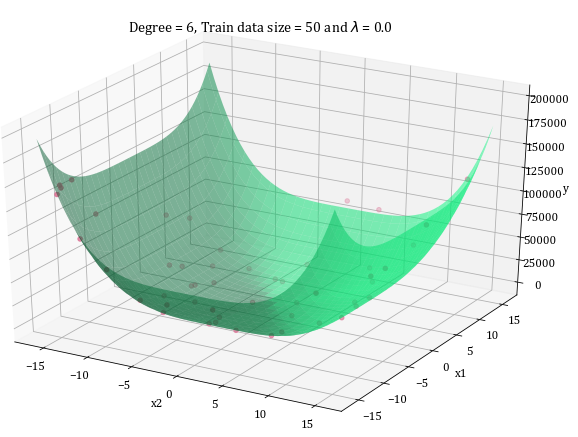
\includegraphics[scale=0.6]{images/D=6,T=50,l=0.0.png}
    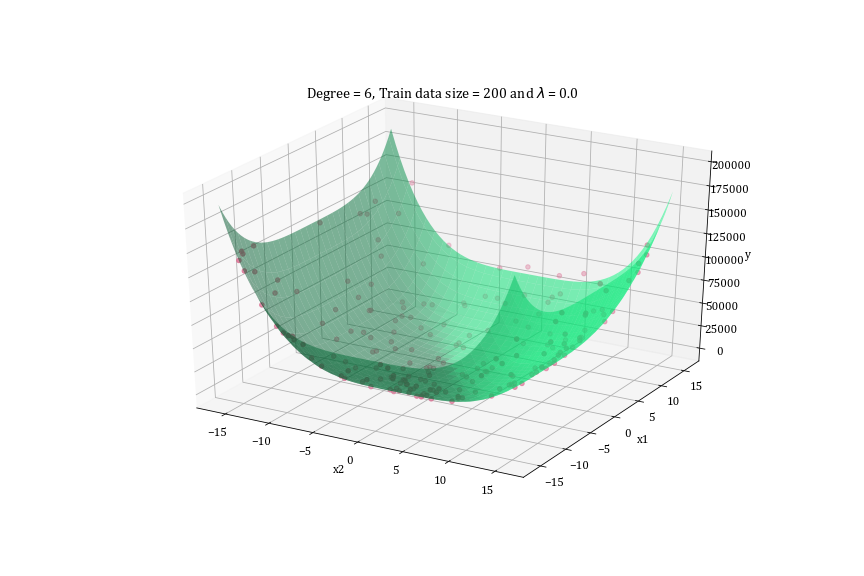
\includegraphics[scale=0.6]{images/D=6,T=200,l=0.0.png}
    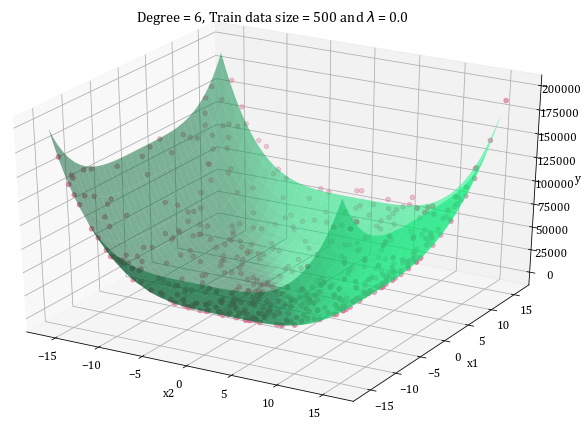
\includegraphics[scale=0.6]{images/D=6,T=500,l=0.0.png}
    \caption{Surface plots of approximated function for different train size, Degree = 6}
    \label{fig:sp_d6}
\end{figure}

\subsubsection{Erms over Train, Validation and Test data}
The $E_{rms}$ values obtained over Train, Validation and Test data are as follows: 
\break

\begin{table}[H]
\centering
\begin{tabular}{l l l l l}
\hline
\hline
\textbf{Train size} & \textbf{$\lambda$} & \textbf{Erms Train} & \textbf{Erms Validation} & \textbf{Erms Test}\\
\hline
\hline
50 & 0 & 7.78*$10^{-8}$ & 3.72*$10^{-7}$ & 6.17*$10^{-7}$  \\
50 & 1 & 1.02*$10^{-4}$ & 1.25*$10^{-3}$ & 2.27*$10^{-3}$ \\
200 & 0 & 1.31*$10^{-8}$ & 1.39*$10^{-8}$ & 1.44*$ 10^{-8}$  \\
500 & 0 & 3.47*$10^{-8}$ & 3.66*$10^{-8}$ & 3.39*$10^{-8}$\\
\hline
\end{tabular}
\caption{Erms for different train sizes for degree of complexity 6}
\end{table}



\subsubsection{Inference}
\begin{itemize}
    \itemsep0em
    \item The complexity of surface in \autoref{fig:sp_d6} has increased significantly compared to that in \autoref{fig:sp_d2} and \autoref{fig:sp_d3}
    \item The $E_{rms}$ values over all the data sets has decreased drastically as compared to the previous models.
    \item While the $E_{rms}$ train is less compared to $E_{rms}$ Validation and $E_{rms}$ Test for train data size = 50, increasing the training data size alleviates this. 
    \item On increasing the train data size to 200, $E_{rms}$ over Train, Validation and Test data all converge to a lower value, signifying an optimum trade off between bias and variance error. Regularization is therefore not required.
    \item On further increasing the Train data size, the $E_{rms}$ increases insignificantly. 
    \item From the above points and cross-validation method, we conclude that the degree of complexity 6 and Train data size of 200 is the optimal model to describe our data, achieving an upper bound Root Mean Squared Error of $~1.5*10^{-8}$ over Train, Validation as well as Test data.
    \item None of the models need to be regularized. On applying regularization, even for very small values of the hyperparameter $\lambda$, the $E_{rms}$ errors increase. 
\end{itemize}


\subsection{Scatter plot of Model output vs Target output}
Using the optimal model of degree 6 and train data size 200, model output vs target output was plotted for both Train and Test data, we find it to closely follow $y-x=0$ line.
\begin{figure}[H]
    \centering
    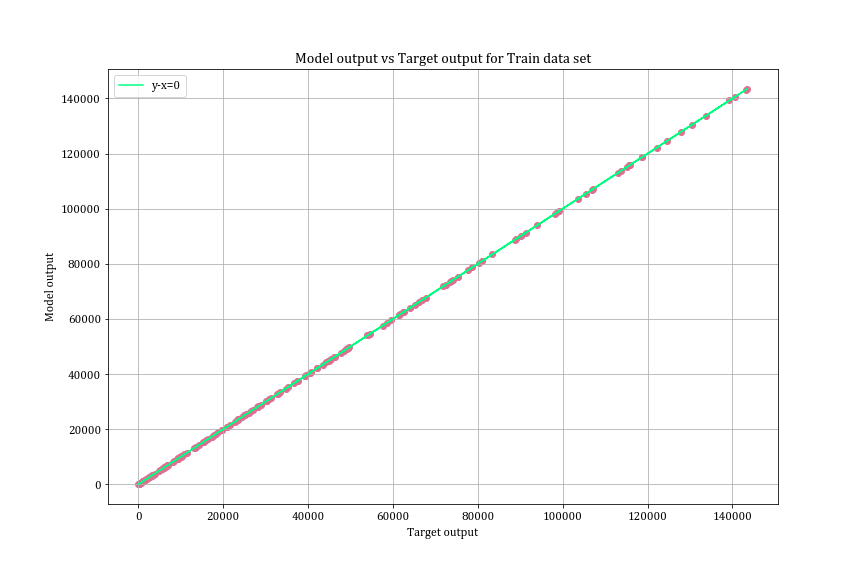
\includegraphics[scale=0.45]{images/tvsy_train.png}
    \caption{Model output against Target output for train dataset.}
    \label{fig:yvst}
\end{figure}

\begin{figure}[H]
    \centering
    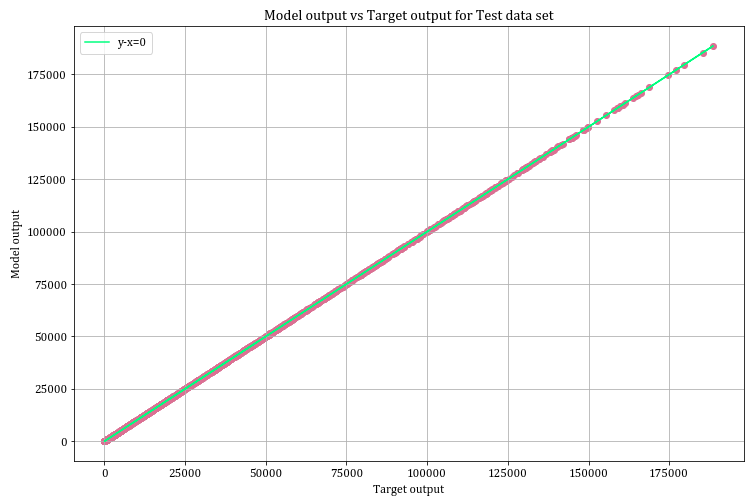
\includegraphics[scale=0.45]{images/tvsy_test.png}
    \caption{Model output against Target output for test dataset.}
\end{figure}

\break
\section{Task 3}
\subsection{Mathematical Formulation}
Linear regression using Gaussian basis function is given as 
\begin{equation}
    y(\vec{x},\vec{w}) = \sum_{i=0}^{D-1} \omega_{i}\phi_{i}(\vec{x})
\end{equation},
where $D$ is a hyperparameter. The basis function 
\begin{equation}
    \phi_{i} = \exp\Big(\frac{-|\vec{x} - \vec{\mu}_i|^2}{\sigma^2}\Big)
\end{equation}
where $i = 1,2 ... D-1$. The $\mu$ are the mean vectors for $D-1$ kernels made from the data set. The value of the mean vectors are found using the KMeans clustering algorithm. In this work, the \tt{sklearn} KMeans function was used.\\

\noi
The Tikhonov regularization term is given by $\vec{\omega}$ = $(\Phi*T\Phi + \lambda \Tilde{\Phi})^{-1} \Phi^T \vec{t}$. The $\Tilde{\Phi}$ term is defined as 
\begin{equation}
    \Tilde{\Phi} = [\Tilde{\phi}]_{i,j = 1}^{K}
\end{equation}
and 
\begin{equation}
    \Tilde{\phi}_{ij} =  \exp\Big(\frac{-|\vec{\mu}_i - \vec{\mu}_j|^2}{\sigma^2}\Big)
\end{equation}

where K is the number of clusters and $\lambda$ is the regularization parameter. 
Running gridsearch on regularization parameter and number of clusters, the result is as given in the table 
a\def\arraystretch{1.25}
\begin{table}[H]
\centering
\begin{tabular}{l l l l l}
\hline
\hline
\textbf{\# Clusters} & \textbf{$\lambda$} & \textbf{RMSE Train} & \textbf{RMSE Validation} & \textbf{RMSE Test}\\
\hline
\hline
17 & 0.0 & 2.9468387558366933 & 1.6547584906306898 & 2.071988832871694\\
20 & 0.0 & 2.8053483856903716 & 1.6793919262797414 & 2.025259227794651\\
18 & 0.0 & 2.8170364466530855 & 1.7038783533934139 & 2.010177058256246\\
16 & 0.0 & 3.3805491988873277 & 2.0535920023124983 & 2.406981516312691\\
15 & 0.0 & 4.548082875715493 & 2.731925954934872 & 3.096909165927102\\
24 & 0.001 & 13.43938595610601 & 8.277187948754543 & 10.036253692369383\\
18 & 0.01 & 14.86361500203557 & 9.043945721398089 & 10.755205727447175\\
25 & 1.0 & 16.38323282900813 & 10.256712214375325 & 11.813474754310901\\
16 & 10.0 & 24.413162366509727 & 15.120135672677915 & 17.144734122954514\\
24 & 100.0 & 27.07933463241804 & 16.715731647995742 & 18.961955749041806\\
\hline
\end{tabular}
\caption{Top 5 RMSE and 5 other representative errors on the Training, Validation and Testing dataset, across different number of clusters, using tikhonov regularization}
\end{table}

\subsection{Dataset 2}
Using Gaussian-basis functions for the regression, three cases of regularization were carried out as follows:

\subsubsection{No Regularization}
With no regularization, the only hyperparameter is the number of clusters. Building models for number of clusters ranging from 1 to 26, the Sum of Squared errors for the train, cross-validation and test data are in \autoref{table:erms_ds2_noreg_gaus}.
\begin{center}
\begin{longtable}{l l l l}
\hline
\hline
\textbf{Number of Clusters} & \textbf{Training Error} & \textbf{CV error} & \textbf{Test error}\\
\hline
\hline
1 & 17.3789 & 10.9059 & 12.9717\\
2 & 17.0904 & 10.6944 & 12.6854\\
3 & 17.0867 & 10.7259 & 12.7264\\
4 & 17.1242 & 10.7506 & 12.7523\\
5 & 14.5314 & 8.7957 & 10.5586\\
6 & 13.3306 & 8.2253 & 10.1263\\
7 & 13.2817 & 8.2313 & 10.1736\\
8 & 13.1093 & 8.1232 & 10.0006\\
9 & 13.1122 & 8.1183 & 9.9791\\
10 & 13.0771 & 8.0986 & 9.9331\\
11 & 8.5937 & 5.4374 & 6.2637\\
12 & 8.1931 & 5.0608 & 5.9119\\
13 & 8.3607 & 5.1849 & 6.0439\\
14 & 7.722 & 4.8476 & 5.4869\\
15 & 4.5496 & 2.7332 & 3.1036\\
16 & 3.4353 & 2.0997 & 2.4499\\
17 & 2.9466 & 1.6523 & 2.071\\
18 & 2.6985 & 1.5286 & 1.9631\\
19 & 3.1347 & 1.8865 & 2.255\\
20 & 3.2905 & 1.8746 & 2.4209\\
21 & 12.8301 & 7.446 & 9.3004\\
22 & 5.2491 & 3.1203 & 3.7844\\
23 & 9.6805 & 5.7236 & 6.9741\\
24 & 14.1133 & 8.0835 & 10.2968\\
25 & 22.9415 & 13.9185 & 16.5549\\
\hline
\caption{RMSE error on dataset 2 using no regularization}
\label{table:erms_ds2_noreg_gaus}
\end{longtable}
\end{center}

\noi
The variation of cross-validation error with the number of clusters is as in \autoref{fig:ds2_noreg_gaus}. We can infer from the table and the figure, the optimal number of clusters is \textbf{20}.
\begin{figure}[H]
    \centering
    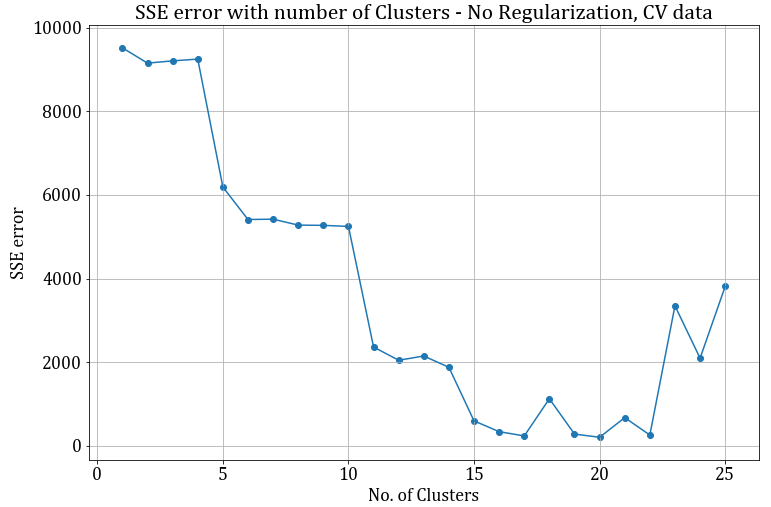
\includegraphics[scale = 0.5]{images/errorplot_ds2_no_reg.png}
    \caption{Plot of CV error with number of clusters, on dataset 2 and no regularization}
    \label{fig:ds2_noreg_gaus}
\end{figure}

\noi
Using the model with 20 clusters on the training and test data, the function in \autoref{fig:surf_ds2_gaus} was built. 

\begin{figure}[H]
    \centering
    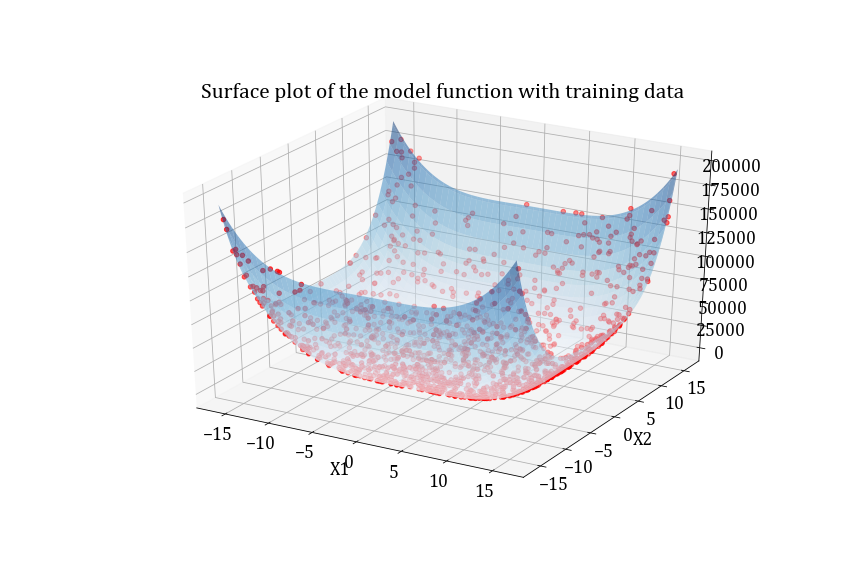
\includegraphics[scale = 0.5]{images/surface_gaus_ds2_noreg.png}
    \caption{Best model of Gaussian basis with no regularization for dataset 2, with training data superimposed.}
    \label{fig:surf_ds2_gaus}
\end{figure}

The performance on training and test data are shown in figure 
\begin{figure}[H]
    \centering
    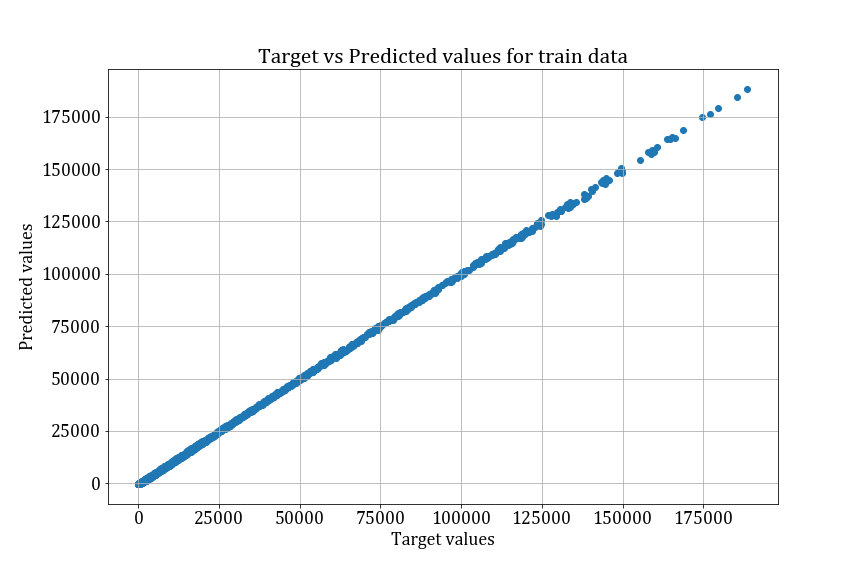
\includegraphics[scale = 0.4]{images/train_ds2_noreg.png}
\end{figure}
\begin{figure}[H]
    \centering
    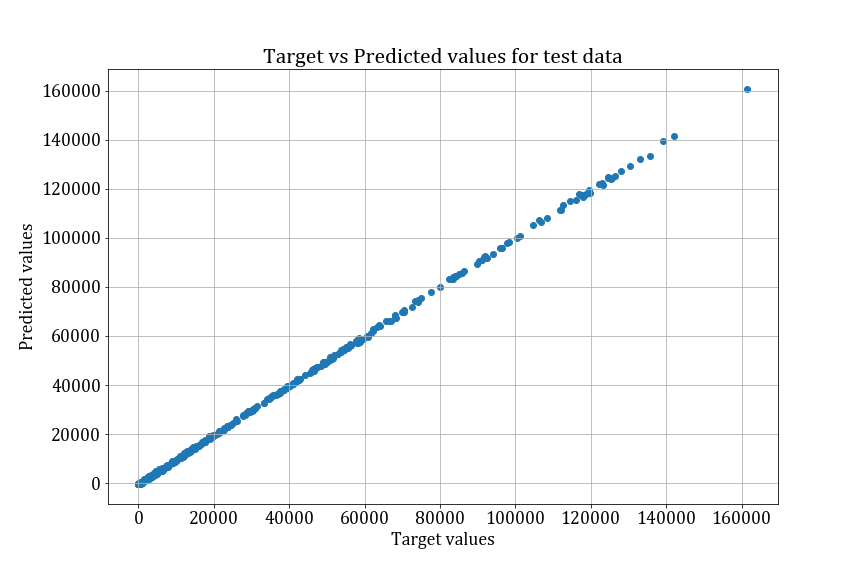
\includegraphics[scale = 0.4]{images/test_ds2_noreg.png}
    \caption{Predictions on train and test data using gaussian basis functions with no regularization on dataset 2}
    \label{fig:train_test_ds2_noreg_gaus}
\end{figure}

\subsubsection{Quadratic regularization}
Performing Quadratic regularization as described in section 2, a gridsearch was performed for the best regularization parameter and number of clusters, as given in table 
\def\arraystretch{1.25}
\begin{table}[H]
\centering
\begin{tabular}{l l l l l}
\hline
\hline
\textbf{\# Clusters} & \textbf{$\lambda$} & \textbf{SSE Train} & \textbf{SSE Validation} & \textbf{SSE Test}\\
\hline
\hline
18 & 0.0 & 14563.95 & 4673.21 & 7707.75\\
20 & 0.0 & 14377.72 & 5204.0 & 7345.81\\
17 & 0.0 & 19580.33 & 6732.68 & 9912.01\\
16 & 0.0 & 22856.23 & 8434.48 & 11587.12\\
19 & 0.0 & 29072.8 & 10207.35 & 15265.15\\
15 & 0.0 & 41578.12 & 14999.85 & 19067.9\\
22 & 0.0 & 74304.87 & 23487.19 & 39912.58\\
14 & 0.0 & 119373.62 & 47199.11 & 60138.86\\
12 & 0.0 & 134254.98 & 51223.42 & 69900.59\\
24 & 0.0 & 138137.32 & 52442.5 & 69461.67\\
\hline
\end{tabular}
\caption{Top 10 SSE on the Training, Validation and Testing dataset, across different number of clusters, using L2 regularization for dataset 2.}
\end{table}

\noi
The best model on validation data does not require any regularization. The optimum number of clusters is similar to the no regularization case of 20. Applying this model on the training and test data, we get the \autoref{fig:gaus_ds2_l2}

\begin{figure}[H]
    \centering
    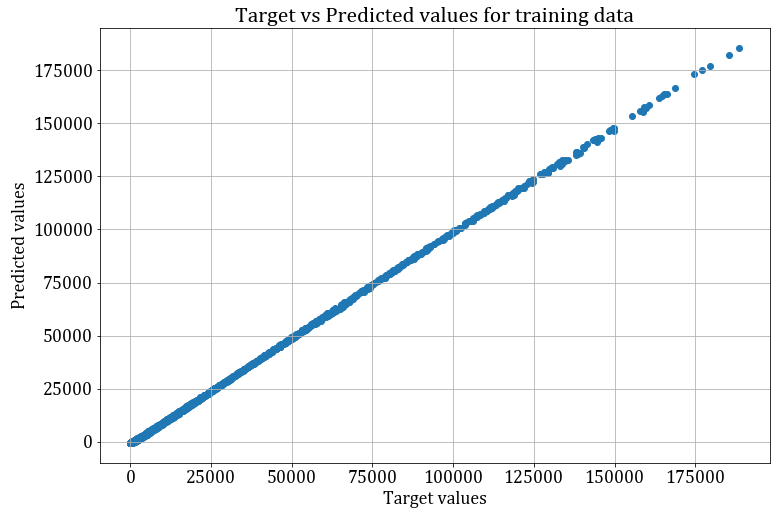
\includegraphics[scale=0.5]{images/train_ds2_L2reg.png}
    \end{figure}
\begin{figure}[H]
    \centering
    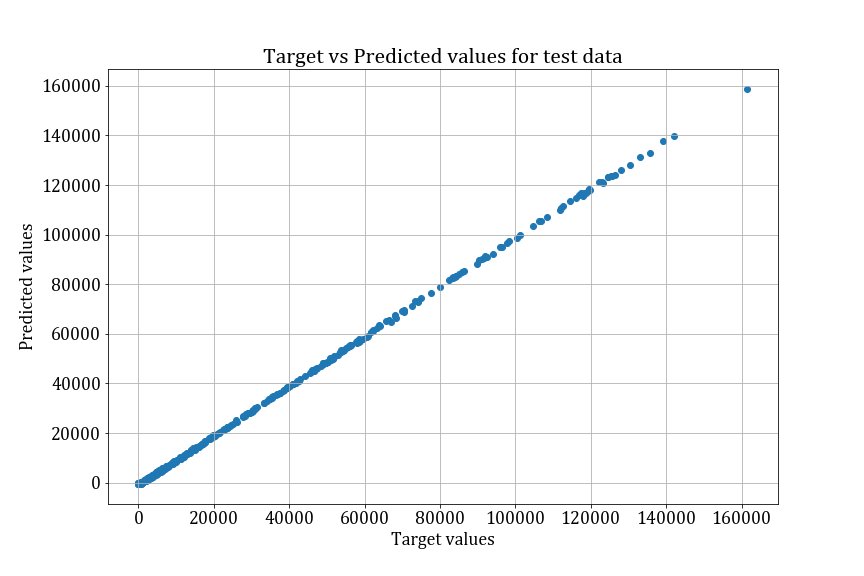
\includegraphics[scale=0.5]{images/test_ds2_L2reg.png}
    \caption{Gaussian basis model with 18 clusters on dataset 2}
    \label{fig:gaus_ds2_l2}
\end{figure}

\subsubsection{Tikhonov regularization}
We can see in the tables that no regularization is required, and the optimal number of clusters is 17 (similar to the previous two cases).
Applying this model on training and test data, we get the \autoref{fig:gaus_ds2_tikh}
\begin{figure}[H]
    \centering
    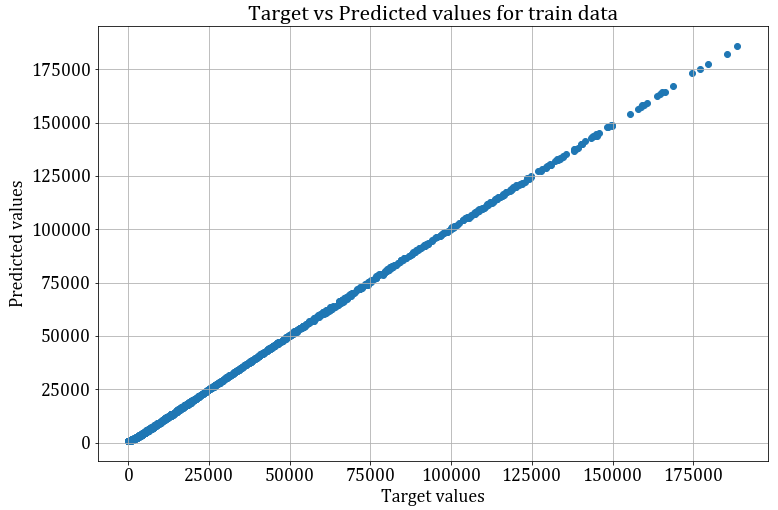
\includegraphics[scale=0.5]{images/train_ds2_tikhreg.png}
\end{figure}
\begin{figure}[H]
    \centering
    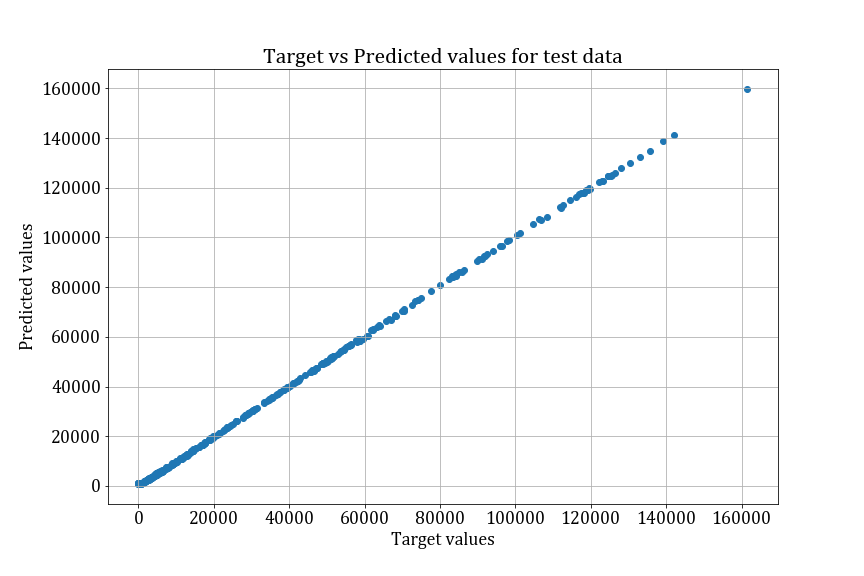
\includegraphics[scale=0.5]{images/test_ds2_tikhreg.png}
    \caption{Gaussian basis model with 17 clusters on dataset 2}
    \label{fig:gaus_ds2_tikh}
\end{figure}

\subsubsection{Inference}
Comparing the different regularization methods, we can see that there is no overfitting on the data. Applying any form regularization on the full data worsens the errors. \\

\noi
\textcolor{blue}{The lowest $E_{rms}$ values obtained are as follows:
\begin{itemize}
    \itemsep0em
    \item Training $E_{rms}$: $1.4786466027685028$
    \item Testing $E_{rms}$: $1.4982621391957776$
\end{itemize}
}

\subsection{Dataset 3}
As the dataset was a real world dataset, the following preprocessing steps were carried out.
\begin{itemize}
    \itemsep0em
    \item \tt{NaN} values: All datapoints that had \tt{NaN} values in any of the columns were removed. 
        \begin{figure}[H]
            \centering
            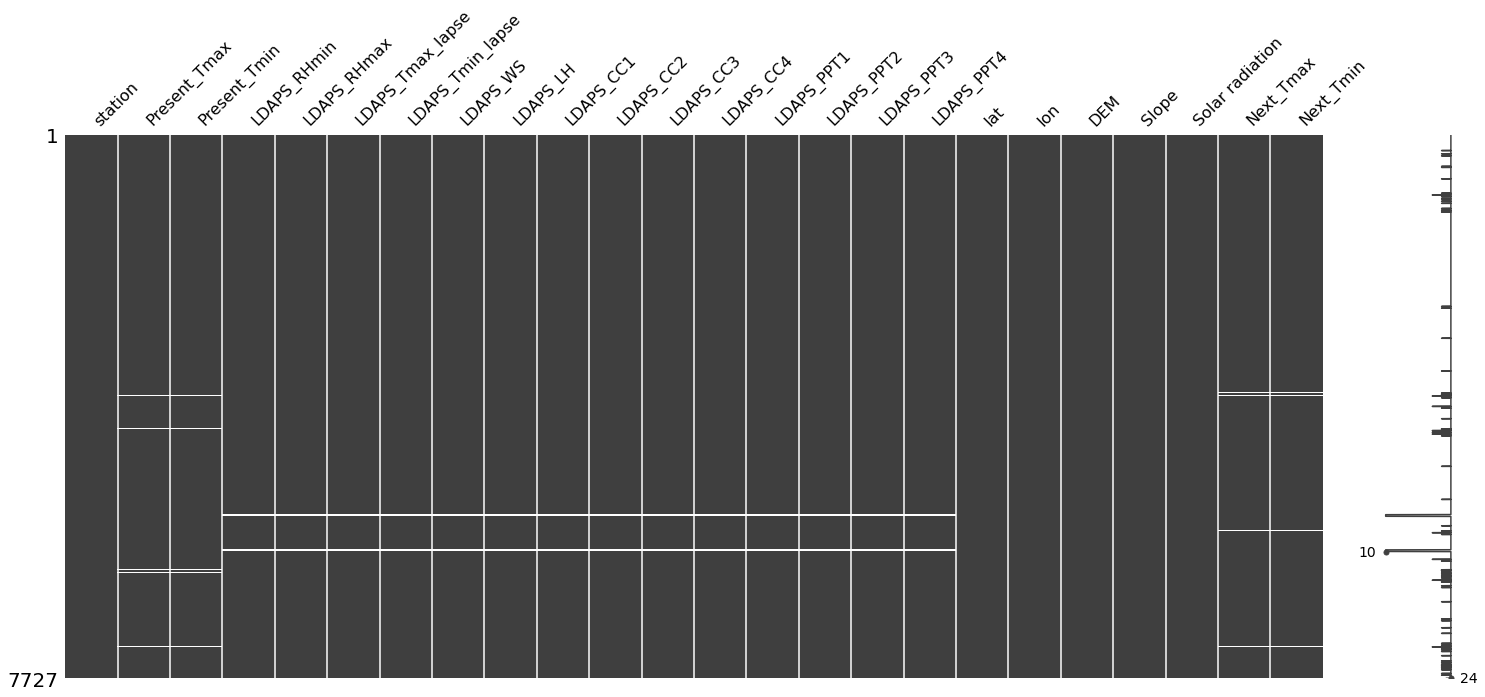
\includegraphics[scale=0.3]{images/missingno.png}
            \caption{Visualization of the original dataset. White lines indicate \tt{NaN}s.}
        \end{figure}

        \begin{figure}[H]
            \centering
            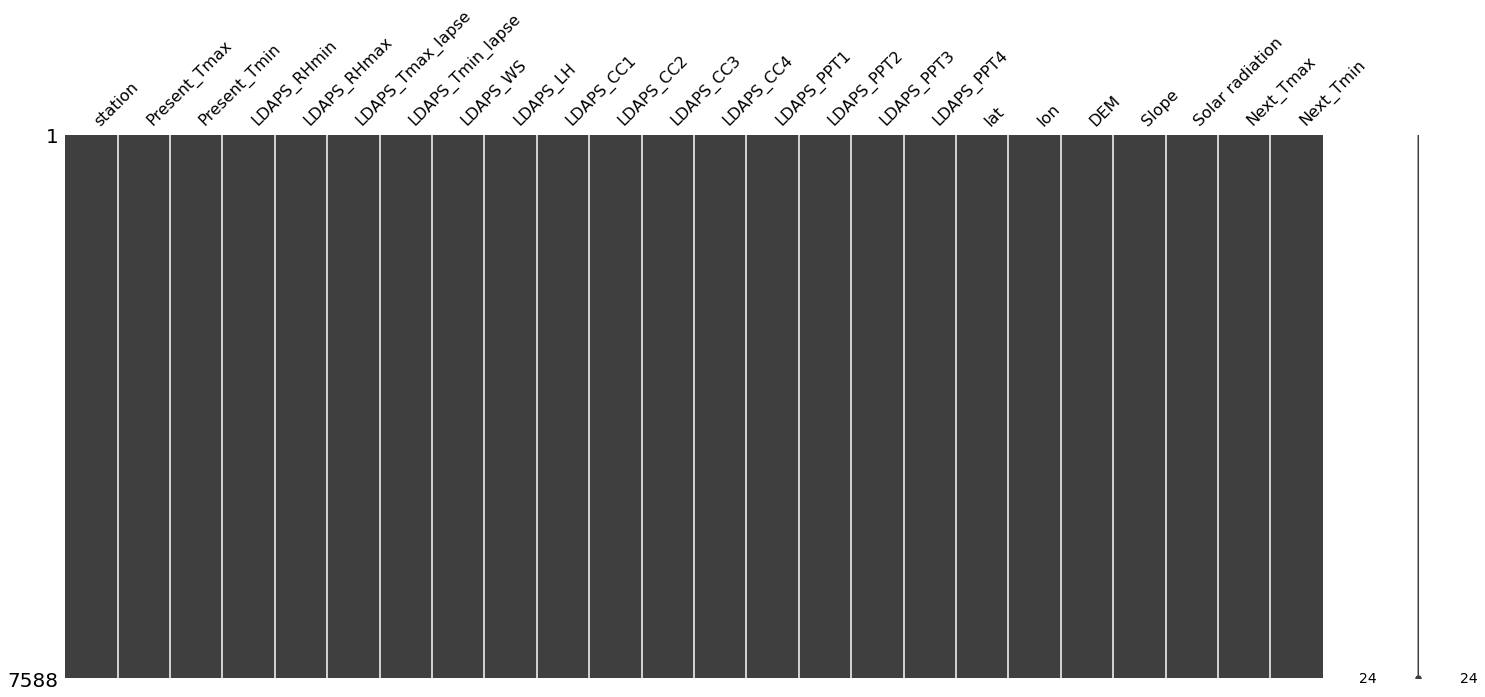
\includegraphics[scale=0.3]{images/cleaned.png}
            \caption{Visualization of the dataset after the removal of \tt{NaN}s.}
        \end{figure}

    \item Highly correlated factors were removed. A threshold of 0.75 was used to identify highly correlated features and they were sequentially removed.
    \item Features that resulted in a high Variance Inflation Factor (VIF) were also removed.
    \item The analysis involving correlated features and VIF was performed on the training data and was then extended to the validation and testing data. 
\end{itemize}


\subsubsection{No Regularization}
The hyperparameter - number of clusters was sweeped and the value that resulted in the lowest validation SSE was chosen. The following cluster numbers were swept for: [1, 2, 3, 4, 5, 6, 7, 8, 9, 15, 20, 25, 30, 40, 50, 60, 70, 80, 90, 100].

\paragraph{Predicting: \tt{Next\_Tmin}}
The $E_{rms}$ on the training and validation dataset and the SSE distances of samples to their closest cluster center obtained across the number of clusters is as follows:
\begin{figure}[H]
     \centering
     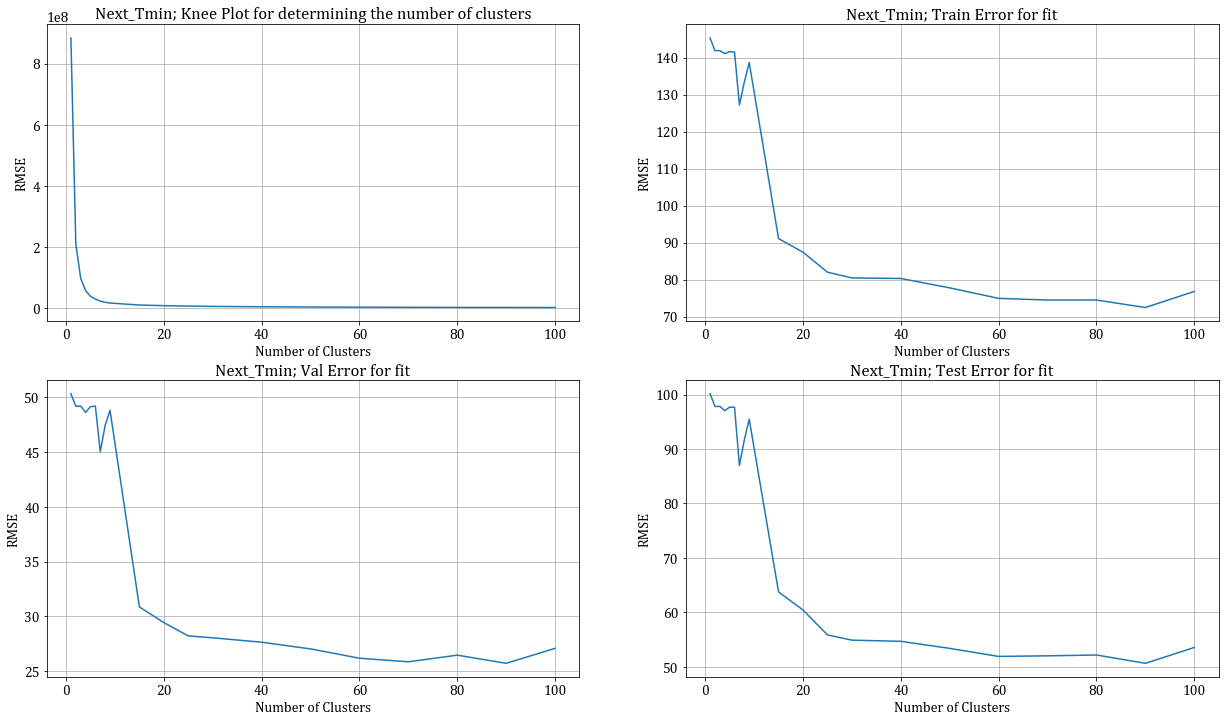
\includegraphics[scale=0.4]{images/t3_d3/no_reg/tmin_errors.png}
     \caption{K-Means inertia, SSE on training and validation data from the left to right respectively.}
\end{figure}

\vspace{-1em}
\noi
The errors obtained in tabular format is as follows:
\def\arraystretch{1.25}
\begin{table}[H]
\centering
\begin{tabular}{l l l l l}
\hline
\hline
\textbf{\# Clusters} & \textbf{Erms Train} & \textbf{Erms Validation} & \textbf{Erms Test}\\
\hline
\hline
90 & 1.0480926961558428 & 1.1145328487370127 & 1.0612317092745545 \\
70 & 1.077282613356503 & 1.1205646601791848 & 1.0900393186117472 \\
60 & 1.0838258289557656 & 1.1347092563134056 & 1.0878633208966022 \\
80 & 1.0773257656133501 & 1.1469280060128313 & 1.0933190935289967 \\
50 & 1.124898166939697 & 1.171619621385478 & 1.1186915649161837 \\
\hline
\end{tabular}
\caption{Erms on the Training, Validation and Testing dataset, across different number of clusters, for 5 hyper parameters that result in the lowest Erms.}
\end{table}


\noi
The the number of clusters that resulted in the lowest RMSE is 90. In addition to the scatter plot, histograms were plotted to understand the variance in the data.\\

\noi
The histogram and scatter plot of the target and the model output is as follows (train data):
\begin{figure}[H]
     \centering
     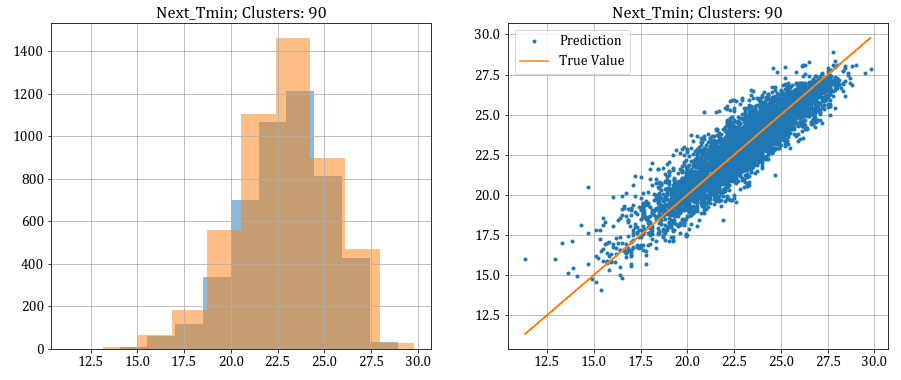
\includegraphics[scale=0.49]{images/t3_d3/no_reg/T_min_nclu_90.png}
     \caption{Histogram and Scatter plot of the target values against the model prediction for training dataset, using linear regression with gaussian basis and $\lambda: 0$}
\end{figure}

\noi
The histogram and scatter plot of the target and the model output is as follows (test data):
\begin{figure}[H]
    \centering
    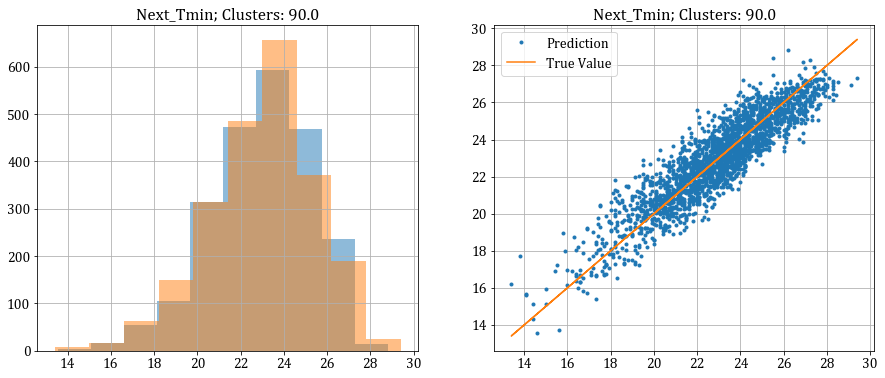
\includegraphics[scale=0.49]{images/t3_d3/no_reg/T_min_test.png}
    \caption{Histogram and Scatter plot of the target values against the model prediction for testing dataset, using linear regression with gaussian basis and $\lambda: 0$}
\end{figure}

\noi
\textcolor{blue}{
The lowest Erms values obtained (number of clusters: 90) are as follows:
\begin{itemize}
    \itemsep0em
    \item Training $E_{rms}$: $1.0480926961558428$
    \item Testing $E_{rms}$: $1.0612317092745545$
\end{itemize}
}

\paragraph{Predicting: \tt{Next\_Tmax}}
The Erms on the training and validation dataset and the RMSE distances of samples to their closest cluster center obtained across the number of clusters is as follows:
\begin{figure}[H]
     \centering
     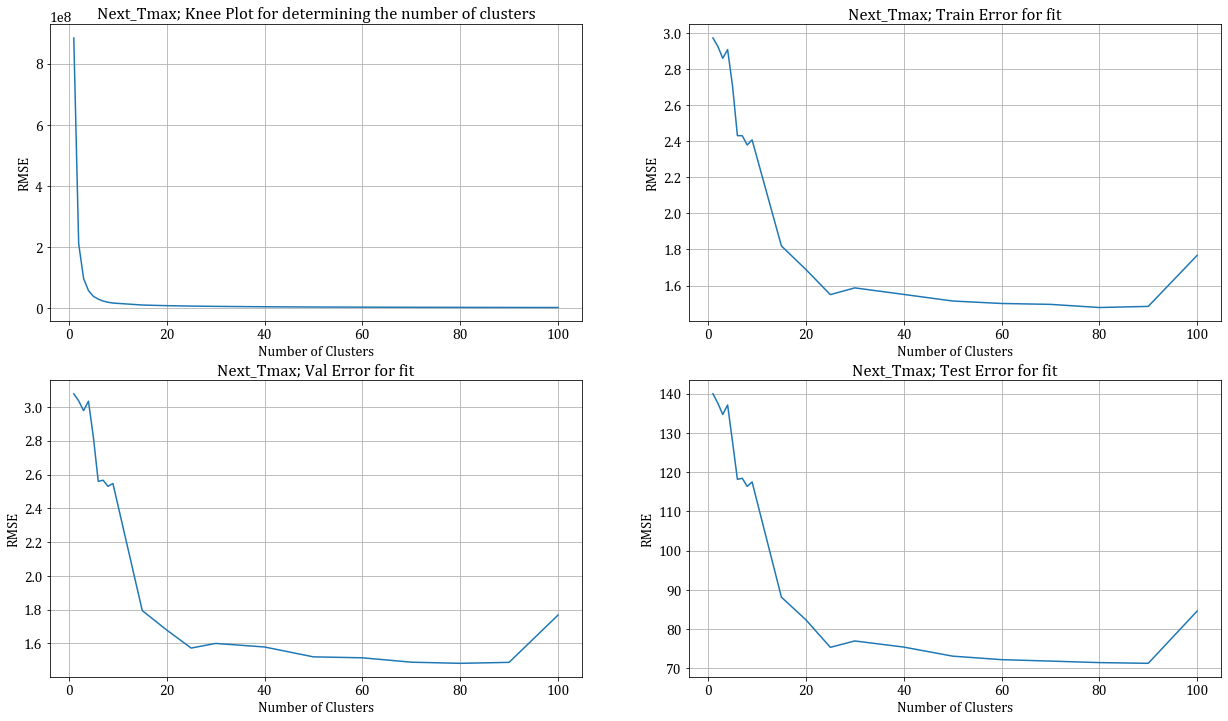
\includegraphics[scale=0.4]{images/t3_d3/no_reg/tmax_errors.png}
     \caption{K-Means inertia, RMSE on training and validation data from the left to right respectively.}
\end{figure}

\vspace{-1em}
\noi
The errors obtained in tabular format is as follows:
\def\arraystretch{1.25}
\begin{table}[H]
\centering
\begin{tabular}{l l l l l}
\hline
\hline
\textbf{\# Clusters} & \textbf{Erms Train} & \textbf{Erms Validation} & \textbf{Erms Test}\\
\hline
\hline
80 & 1.48 & 1.48 & 1.50 \\
90 & 1.48 & 1.49 & 1.49 \\
70 & 1.50 & 1.49 & 1.51 \\
60 & 1.50 & 1.52 & 1.51 \\
50 & 1.51 & 1.52 & 1.53 \\
\hline
\end{tabular}
\caption{Erms on the Training, Validation and Testing dataset, across different number of clusters, for 5 hyper parameters that result in the lowest Erms.}
\end{table}


\noi
The the number of clusters that resulted in the lowest RMSE is 80. In addition to the scatter plot, histograms were plotted to understand the variance in the data.\\

\noi
The histogram and scatter plot of the target and the model output is as follows (train data):
\begin{figure}[H]
     \centering
     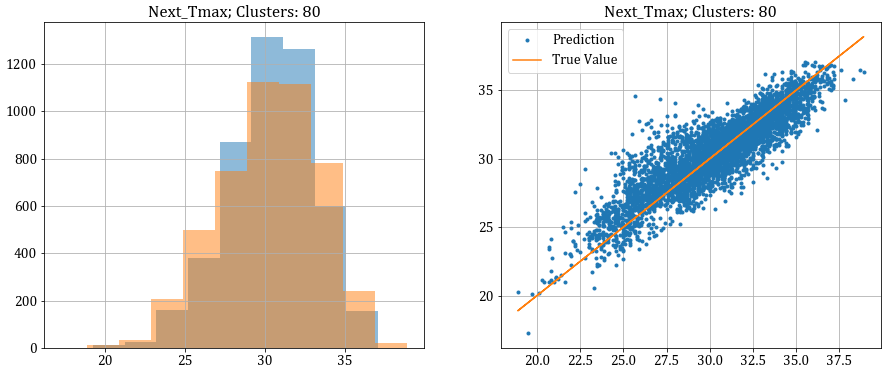
\includegraphics[scale=0.49]{images/t3_d3/no_reg/T_max_nclu_80.png}
     \caption{Histogram and Scatter plot of the target values against the model prediction for training dataset, using linear regression with gaussian basis and $\lambda: 0$}
\end{figure}

\noi
The histogram and scatter plot of the target and the model output is as follows (test data):
\begin{figure}[H]
    \centering
    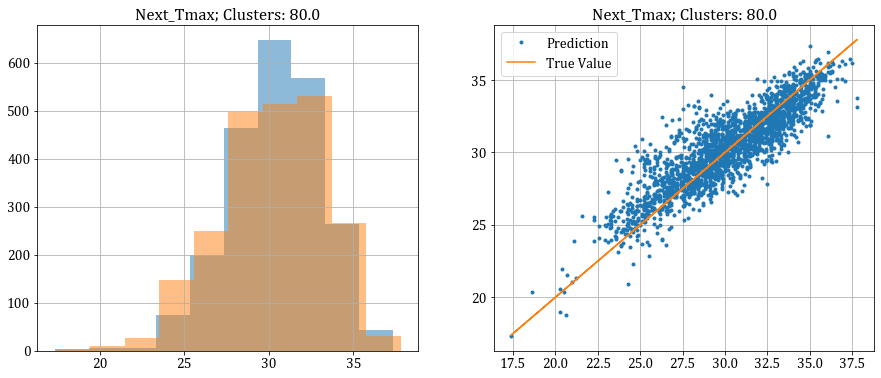
\includegraphics[scale=0.49]{images/t3_d3/no_reg/T_max_test.png}
    \caption{Histogram and Scatter plot of the target values against the model prediction for testing dataset, using linear regression with gaussian basis and $\lambda: 0$}
\end{figure}

\noi
\textcolor{blue}{The lowest $E_{rms}$ values obtained (number of clusters: 80) are as follows:
\begin{itemize}
    \itemsep0em
    \item Training $E_{rms}$: $1.4786466027685028$
    \item Testing $E_{rms}$: $1.4982621391957776$
\end{itemize}
}

\subsubsection{Quadratic Regularization}
Optimal parameters using quadratic regularization is given by $\vec{\omega^*}$ = $(\Phi^T\Phi + \lambda I)^{-1} \Phi^T \vec{t}$;\\

\noi
$\lambda$ is the regularization parameter. The RMSE on the cross-validation set was calculated for each value. The best performing model was selected as the one having least RMSE on CV data \\

\noi
The hyperparameter - number of clusters and $\lambda$ were sweeped and the value that resulted in the lowest validation SSE was chosen. The following cluster numbers were swept for: [1, 2, 3, 4, 5, 6, 7, 8, 9, 15, 20, 25, 30, 40, 50, 60, 70, 80, 90, 100] and the following $\lambda$ values were sweeped: [0.01, 0.1,  1.0, 5.0, 10.0].

\paragraph{Predicting: \tt{Next\_Tmin}}
The Erms on the training and validation dataset and the SSE distances of samples to their closest cluster center obtained across the number of clusters is as follows:
\def\arraystretch{1.25}
\begin{table}[H]
\centering
\begin{tabular}{l l l l l}
\hline
\hline
\textbf{\# Clusters} & \textbf{$\lambda$} & \textbf{$E_{rms}$ Train} & \textbf{$E_{rms}$ Validation} & \textbf{$E_{rms}$ Test}\\
\hline
\hline
200 & 0.01 & 1.9013040128753353 & 1.9965582216927813 & 1.9047855943641792 \\
190 & 0.01 & 1.904933411245413 & 1.9990574601548905 & 1.908742610287438 \\
180 & 0.01 & 1.906872845452907 & 1.9994072596187717 & 1.9109215864242062 \\
170 & 0.01 & 1.916154510430869 & 2.007065870193715 & 1.9205837284324376 \\
160 & 0.01 & 1.9265592590375111 & 2.0159961584465105 & 1.9311538203795762 \\
\hline
\end{tabular}
\caption{$E_{rms}$ on the Training, Validation and Testing dataset, across different number of clusters, for 5 hyper parameters that result in the lowest $E_{rms}$.}
\end{table}


\noi
The the number of clusters that resulted in the lowest RMSE is 200 and $\lambda$ is $0.01$. In addition to the scatter plot, histograms were plotted to understand the variance in the data.\\

\noi
The histogram and scatter plot of the target and the model output is as follows (train data):
\begin{figure}[H]
     \centering
     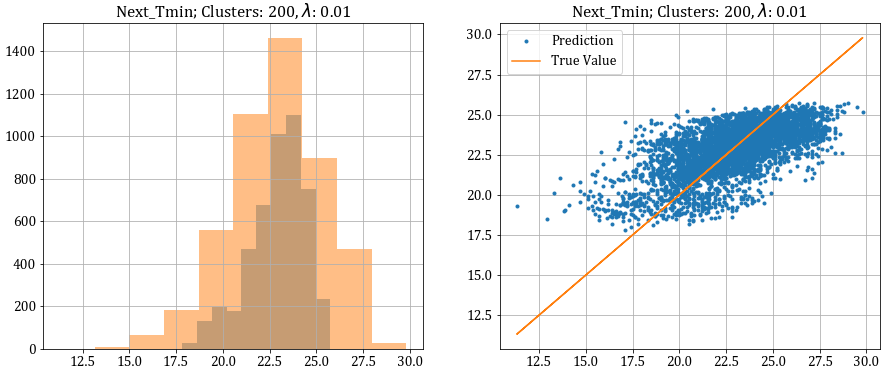
\includegraphics[scale=0.49]{images/t3_d3/reg/T_min_nclu_200_lambda_0.01.png}
     \caption{Histogram and Scatter plot of the target values against the model prediction for training dataset, using linear regression with gaussian basis and $\lambda: 0.01$}
\end{figure}

\noi
The histogram and scatter plot of the target and the model output is as follows (test data):
\begin{figure}[H]
    \centering
    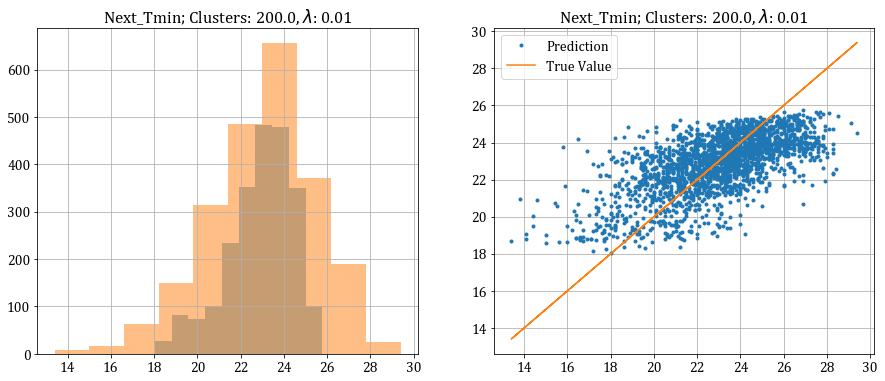
\includegraphics[scale=0.49]{images/t3_d3/reg/tmin_test.png}
    \caption{Histogram and Scatter plot of the target values against the model prediction for testing dataset, using linear regression with gaussian basis and $\lambda: 0.01$}
\end{figure}

\noi
The lowest Erms values obtained are as follows:
\begin{itemize}
    \itemsep0em
    \item Training $E_{rms}$: $1.9013040128753353$
    \item Testing $E_{rms}$: $1.9047855943641792$
\end{itemize}

\paragraph{Predicting: \tt{Next\_Tmax}}
The Erms on the training and validation dataset and the RMSE distances of samples to their closest cluster center obtained across the number of clusters is as follows:
\def\arraystretch{1.25}
\begin{table}[H]
\centering
\begin{tabular}{l l l l l}
\hline
\hline
\textbf{\# Clusters} & \textbf{$\lambda$} & \textbf{Erms Train} & \textbf{Erms Validation} & \textbf{Erms Test}\\
\hline
\hline
200 & 0.01 & 2.249936156869166 & 2.399288774682482 & 2.302560104383557 \\
190 & 0.01 & 2.2523172411109824 & 2.4004581548123065 & 2.3045855076045143 \\
180 & 0.01 & 2.2602647948690384 & 2.4079528711983964 & 2.313110392501987 \\
170 & 0.01 & 2.2640439964624384 & 2.4103143785285273 & 2.3164194038569397 \\
160 & 0.01 & 2.2690106265072445 & 2.414998730544044 & 2.32150961586746 \\
\hline
\end{tabular}
\caption{Erms on the Training, Validation and Testing dataset, across different number of clusters, for 5 hyper parameters that result in the lowest Erms.}
\end{table}


\noi
The the number of clusters that resulted in the lowest RMSE is 200 and $\lambda$ is $0.01$. In addition to the scatter plot, histograms were plotted to understand the variance in the data.\\

\noi
The histogram and scatter plot of the target and the model output is as follows (train data):
\begin{figure}[H]
     \centering
     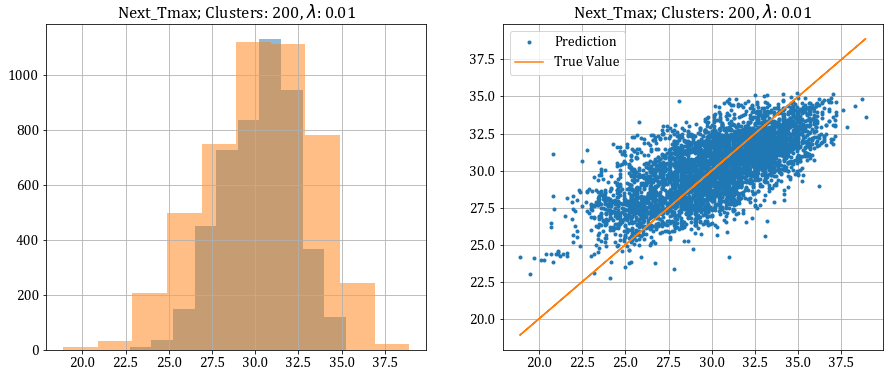
\includegraphics[scale=0.49]{images/t3_d3/reg/T_max_nclu_200_lambda_0.01.png}
     \caption{Histogram and Scatter plot of the target values against the model prediction for training dataset, using linear regression with gaussian basis and $\lambda: 0.01$}
\end{figure}

\noi
The histogram and scatter plot of the target and the model output is as follows (test data):
\begin{figure}[H]
    \centering
    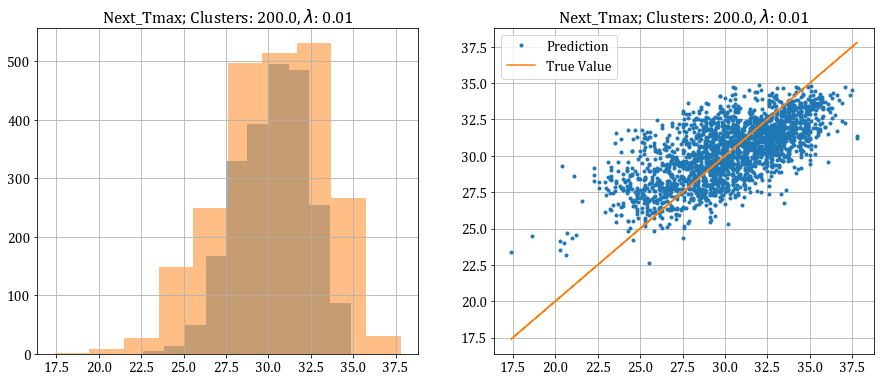
\includegraphics[scale=0.49]{images/t3_d3/reg/tmax_test.png}
    \caption{Histogram and Scatter plot of the target values against the model prediction for testing dataset, using linear regression with gaussian basis and $\lambda: 0.01$}
\end{figure}

\noi
\textcolor{blue}{
The lowest Erms values obtained are as follows:
\begin{itemize}
    \itemsep0em
    \item Training $E_{rms}$: $2.249936156869166$
    \item Testing $E_{rms}$: $2.302560104383557$
\end{itemize}
}

\subsubsection{Tikhonov Regularization} 
As defined in section 3.1, tikhonov regularization was applied to data set 3. Using the regularization coefficient and number of clusters as hyperparameters, gridsearch was done on the train, validation and test set and the model performing best on validation set was chosen. 
\paragraph{Predicting: \tt{Next\_Tmin}}
The following table gives the Erms using different combinations of hyperparameter values:

\def\arraystretch{1.25}
\begin{table}[H]
\centering
\begin{tabular}{l l l l l}
\hline
\hline
\textbf{\# Clusters} & \textbf{$\lambda$} & \textbf{$E_{rms}$ Train} & \textbf{$E_{rms}$ Validation} & \textbf{$E_{rms}$ Test}\\
\hline
\hline
90 & 10.0 & 1.038 & 1.102 & 1.063\\
80 & 5.0 & 1.049 & 1.11 & 1.066\\
80 & 0.1 & 1.054 & 1.111 & 1.068\\
90 & 0.01 & 1.055 & 1.112 & 1.083\\
70 & 1.0 & 1.06 & 1.113 & 1.068\\
100 & 1.0 & 1.065 & 1.114 & 1.077\\
70 & 0.01 & 1.061 & 1.114 & 1.069\\
70 & 5.0 & 1.059 & 1.116 & 1.068\\
90 & 5.0 & 1.073 & 1.116 & 1.095\\
\hline
\end{tabular}
\caption{$E_{rms}$ on the Training, Validation and Testing dataset, across different number of clusters, for 5 hyper parameters that result in the lowest $E_{rms}$, using Tikhonov regularization for \tt{Next\_Tmin}.}
\end{table}
As seen in the table, the optimum value of the hyperparameters for  \tt{Next\_Tmin} is \textbf{90} clusters and $\lambda$ value of \textbf{10}. Using these values on the training and test data gives us the scatter plots in \autoref{fig:ds3_tikh_min}
\begin{figure}
    \centering
    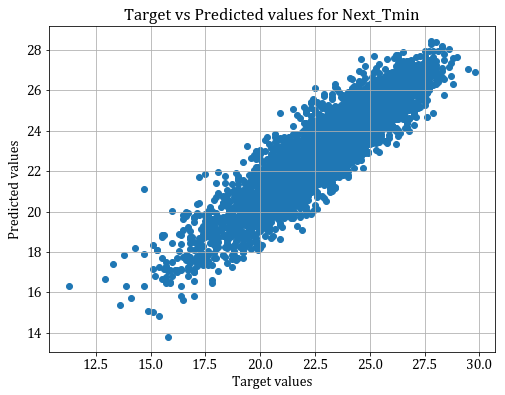
\includegraphics[scale = 0.4]{images/train_ds3_tikh_min.png}
    \includegraphics[scale = 0.4]{images/test_ds3_tikh_min.png}
    \caption{Gaussian basis model on dataset3 using tikhonov regularization for \tt{Next\_Tmin}}
    \label{fig:ds3_tikh_min}
\end{figure}
The lowest Erms values obtained are as follows:
\begin{itemize}
    \itemsep0em
    \item Training $E_{rms}$: $1.038$
    \item Testing $E_{rms}$: $1.063$
\end{itemize}
\paragraph{Predicting: \tt{Next\_Tmax}}
The following table gives the Erms using different combinations of hyperparameter values:

\def\arraystretch{1.25}
\begin{table}[H]
\centering
\begin{tabular}{l l l l l}
\hline
\hline
\textbf{\# Clusters} & \textbf{$\lambda$} & \textbf{$E_{rms}$ Train} & \textbf{$E_{rms}$ Validation} & \textbf{$E_{rms}$ Test}\\
\hline
\hline
90 & 0.01 & 1.454 & 1.467 & 1.474\\
90 & 5.0 & 1.444 & 1.469 & 1.466\\
80 & 0.1 & 1.473 & 1.477 & 1.491\\
80 & 5.0 & 1.48 & 1.479 & 1.505\\
90 & 10.0 & 1.464 & 1.482 & 1.497\\
80 & 0.01 & 1.475 & 1.483 & 1.504\\
90 & 1.0 & 1.47 & 1.484 & 1.497\\
70 & 5.0 & 1.472 & 1.484 & 1.493\\
70 & 0.1 & 1.468 & 1.485 & 1.49\\
70 & 0.01 & 1.477 & 1.486 & 1.497\\
\hline
\end{tabular}
\caption{$E_{rms}$ on the Training, Validation and Testing dataset, across different number of clusters, for 5 hyper parameters that result in the lowest $E_{rms}$, using Tikhonov regularization for \tt{Next\_Tmax}.}
\end{table}

As seen in the table, the optimum value of the hyperparameters for  \tt{Next\_Tmax} is \textbf{90} clusters and $\lambda$ value of \textbf{0.01}. Using these values on the training and test data gives us the scatter plots in \autoref{fig:ds3_tikh_max}
\begin{figure}
    \centering
    \includegraphics[scale = 0.4]{images/train_ds3_tikh_max.png}
    \includegraphics[scale = 0.4]{images/test_ds3_tikh_max.png}
    \caption{Gaussian basis model on dataset3 using tikhonov regularization for \tt{Next\_Tmax}}
    \label{fig:ds3_tikh_max}
\end{figure}

\textcolor{blue}{
\noi
The lowest Erms values obtained are as follows:
\begin{itemize}
    \itemsep0em
    \item Training $E_{rms}$: $1.454$
    \item Testing $E_{rms}$: $1.474$
\end{itemize}
}

\subsubsection{Inference}
From the above plots we observe that:
\begin{itemize}
    \itemsep0em
    \item The model predictions are better when Tikhonov regularization is applied. The $E_{rms}$ when quadratic regularization is applied is marginally higher than when $\lambda$ is 0.
    \item The predictions of the model is better when the number of clusters considered is larger and hence, the $E_{rms}$ is smaller.
    \item In case of no-regularization, we observed that the training, validation and testing $E_{rms}$ increased at the highest number of clusters considered. This could be potentially due to improper initialization.
    \item In addition we see that the variance in the prediction is lower when the number of clusters considered is lower. This can be observed in the plots below:
    \begin{figure}[H]
        \centering
        \includegraphics[scale=0.4]{images/t3_d3/no_reg/T_max_nclu_1.png}
        \caption{Histogram and Scatter plot of the target values against the model prediction for training dataset, using linear regression with gaussian basis and $\lambda: 0$}
    \end{figure}
    \begin{figure}[H]
        \centering
        \includegraphics[scale=0.4]{images/t3_d3/no_reg/T_max_nclu_5.png}
        \caption{Histogram and Scatter plot of the target values against the model prediction for training dataset, using linear regression with gaussian basis and $\lambda: 0$}
    \end{figure}
    \begin{figure}[H]
        \centering
        \includegraphics[scale=0.4]{images/t3_d3/no_reg/T_max_nclu_15.png}
        \caption{Histogram and Scatter plot of the target values against the model prediction for training dataset, using linear regression with gaussian basis and $\lambda: 0$}
    \end{figure}

    \begin{figure}[H]
        \centering
        \includegraphics[scale=0.4]{images/t3_d3/reg/T_max_nclu_1_lambda_0.01.png}
        \caption{Histogram and Scatter plot of the target values against the model prediction for training dataset, using linear regression with gaussian basis and $\lambda: 0.1$}
    \end{figure}
    \begin{figure}[H]
        \centering
        \includegraphics[scale=0.4]{images/t3_d3/reg/T_max_nclu_20_lambda_0.01.png}
        \caption{Histogram and Scatter plot of the target values against the model prediction for training dataset, using linear regression with gaussian basis and $\lambda: 0.1$}
    \end{figure}
    \begin{figure}[H]
        \centering
        \includegraphics[scale=0.4]{images/t3_d3/reg/T_max_nclu_200_lambda_0.01.png}
        \caption{Histogram and Scatter plot of the target values against the model prediction for training dataset, using linear regression with gaussian basis and $\lambda: 0.1$}
    \end{figure}
\end{itemize}
\end{document}